\chapter{Experiments}
\label{experiments_chapter}
In this chapter, we will evaluate the performance of the various agents when confronted with different combinations of obstacles, as well as presenting interesting observations made during the experiments. One of the key questions we aim to answer is whether any of the agents are a are capable of learning to play the entire game.

\section{Individual traps environments}
This section discusses the performance of agents in environments containing only one trap at a time.

\begin{figure}[h]
    \centering
    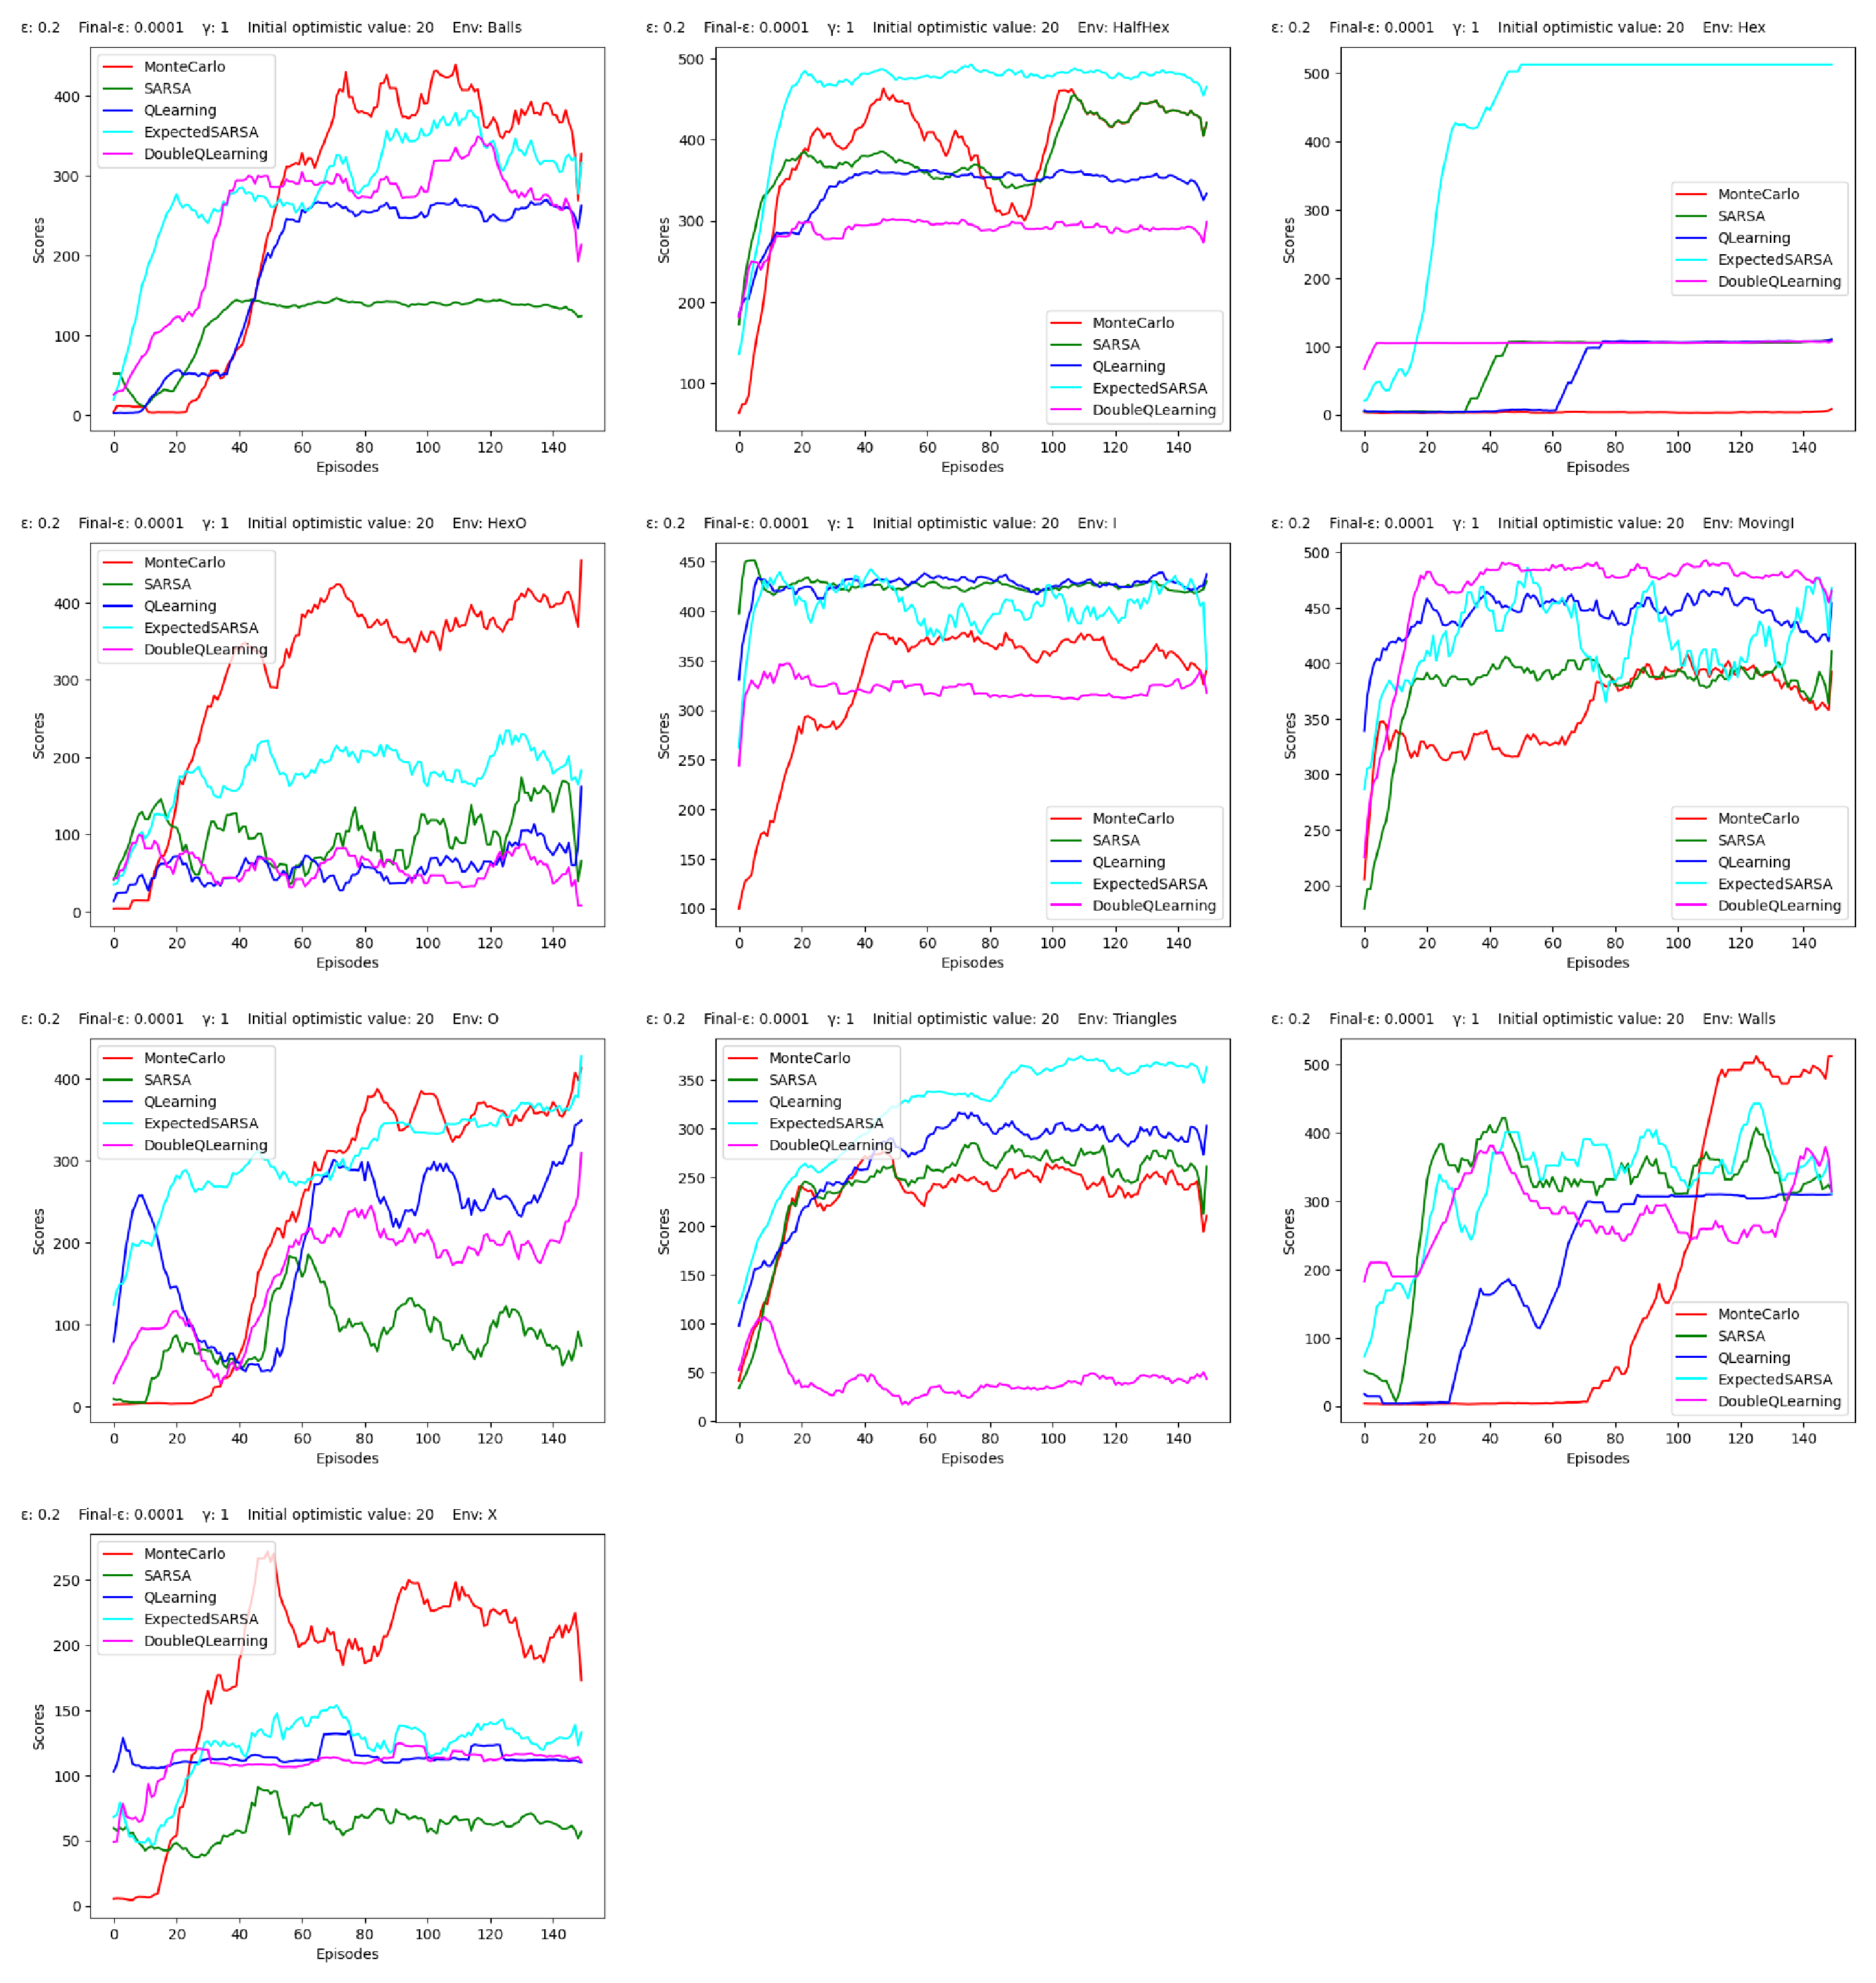
\includegraphics[width=\textwidth]{all_traps}
    \caption{Individual traps examples}
    \label{fig:all_traps}
\end{figure}

Immediately in Figure \ref{fig:all_traps}, for each trap, there is a plot with \texttt{eps=0.2} and \texttt{initOptVal=20} and how each agent performed in this case. These values were picked because with most traps the agents performed well under these conditions.

It should be noted that all plots within this section have smoothing applied with \texttt{window=10}. Thus certain spikes are not be visible. Additionally, unless otherwise suggested, you can assume that the values that were produced are an average of 5 different seeds. The aim is to show a realistic picture on how the agent would perform, and not show the occurrences in which the outcome was satisfactory but rather account for the failures in reproducing the perfect policy as well.

In some cases, of course, the hyperparameters used for plotting Figure \ref{fig:all_traps} were not ideal. However, for most trap/agent pairs, we managed to find at least one combination of hyperparameters where the agent found an optimal or decent policy across multiple seeds. The only exceptions were the \texttt{MonteCarlo} agent with the \texttt{Hex} trap, \texttt{DoubleQLearning} with \texttt{HexO}, \texttt{Triangles}, and \texttt{X} traps, and \texttt{SARSA} and \texttt{QLearning} with \texttt{HexO} trap. \texttt{ExpectedSARSA} was the only agent that produced satisfactory results for all individual trap types and even performed exceptionally well with certain hyperparameters for the \texttt{Hex}, \texttt{I}, \texttt{MovingI}, \texttt{O}, and \texttt{Walls} traps, in which cases it found an optimal policy across multiple seed values.

\begin{figure}[h]
    \centering
    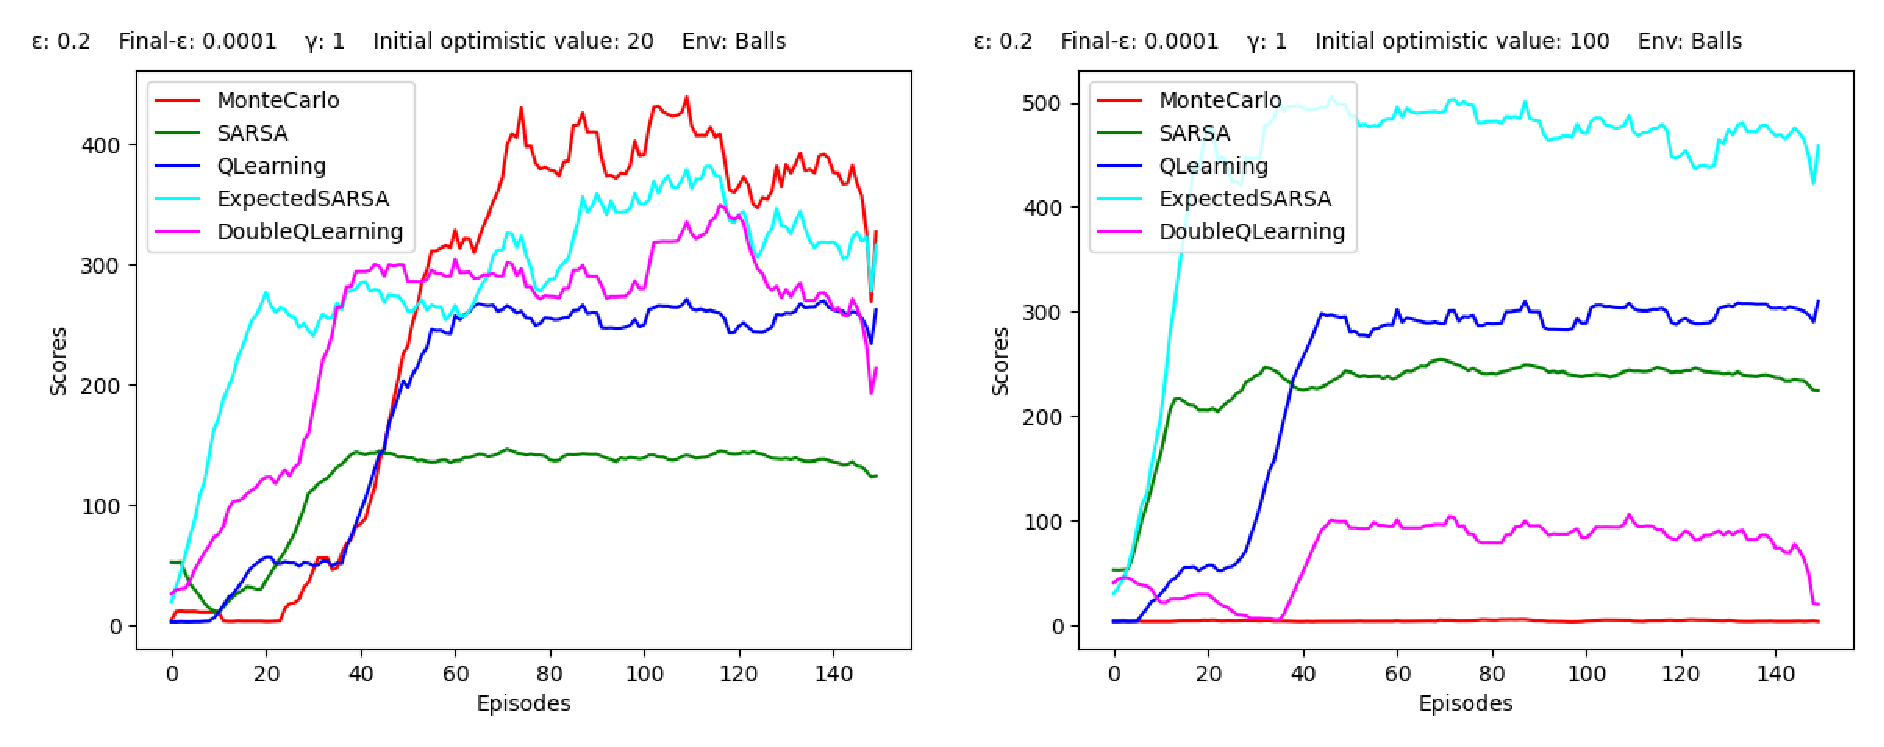
\includegraphics[width=\textwidth]{balls}
    \caption{\texttt{Balls} trap examples}
    \label{fig:balls_eg}
\end{figure}

Choices of the hyperparameters are a very important factor. Most the commonly values in this section are \texttt{eps=0.2} and \texttt{initOptVal=20.0}\\ or \texttt{initOptVal=100.0}. A good example of how much hyperparameters can influence the outcome visible in Figure \ref{fig:balls_eg}. The \texttt{Balls} trap varies significantly based on the initial optimistic value used. This plot underscores the importance of carefully selecting hyperparameters when training reinforcement learning.

\begin{figure}[h]
    \centering
    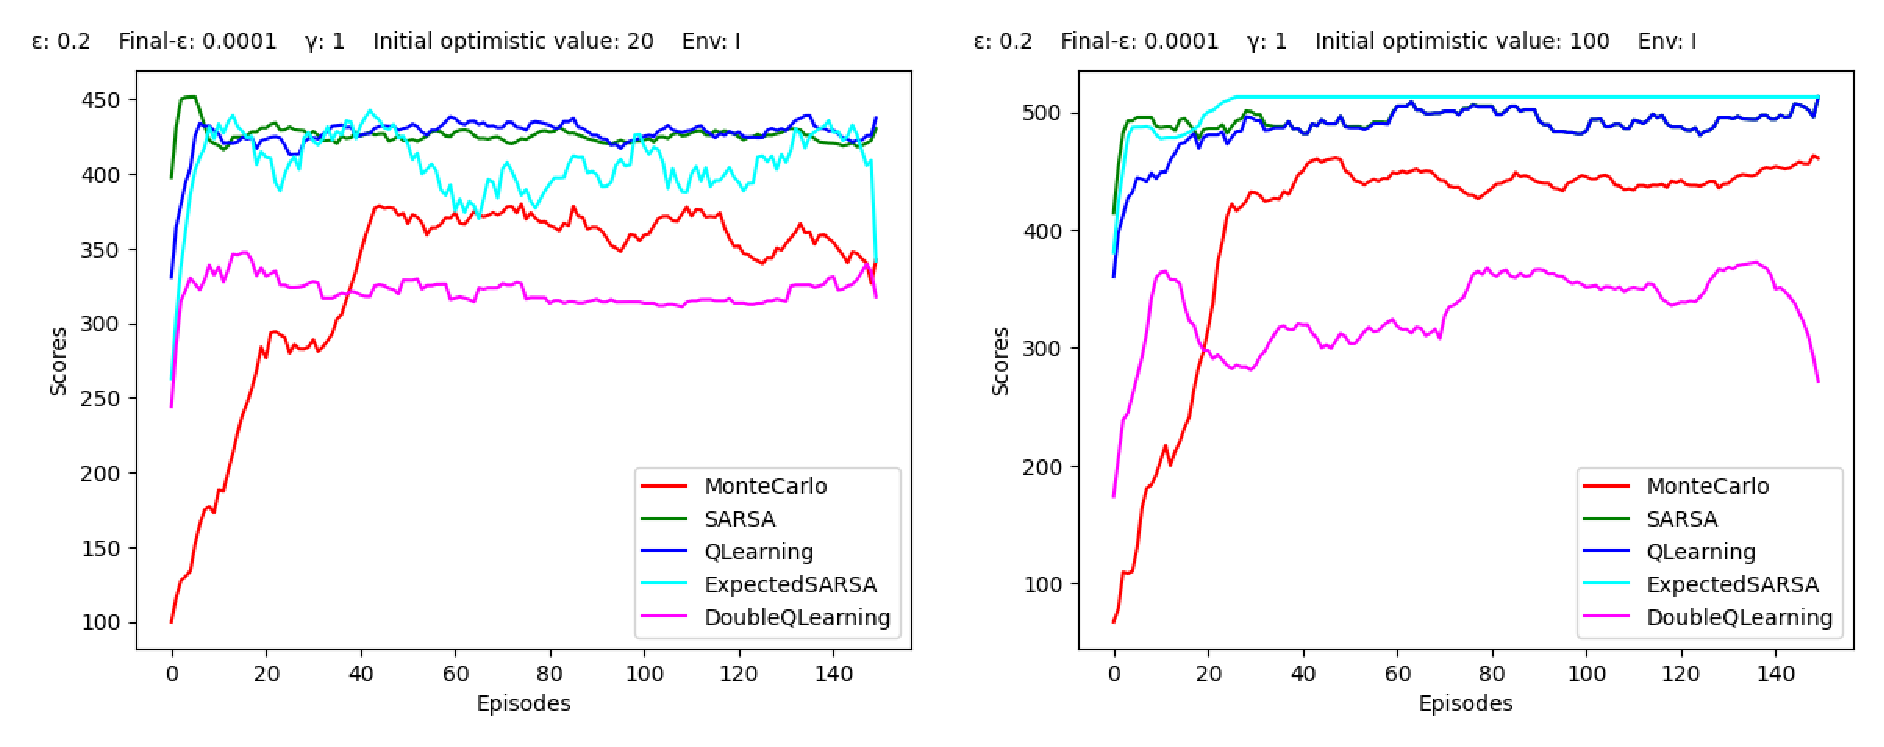
\includegraphics[width=\textwidth]{i}
    \caption{\texttt{I} trap examples}
    \label{fig:i_eg}
\end{figure}

\begin{figure}[h]
    \centering
    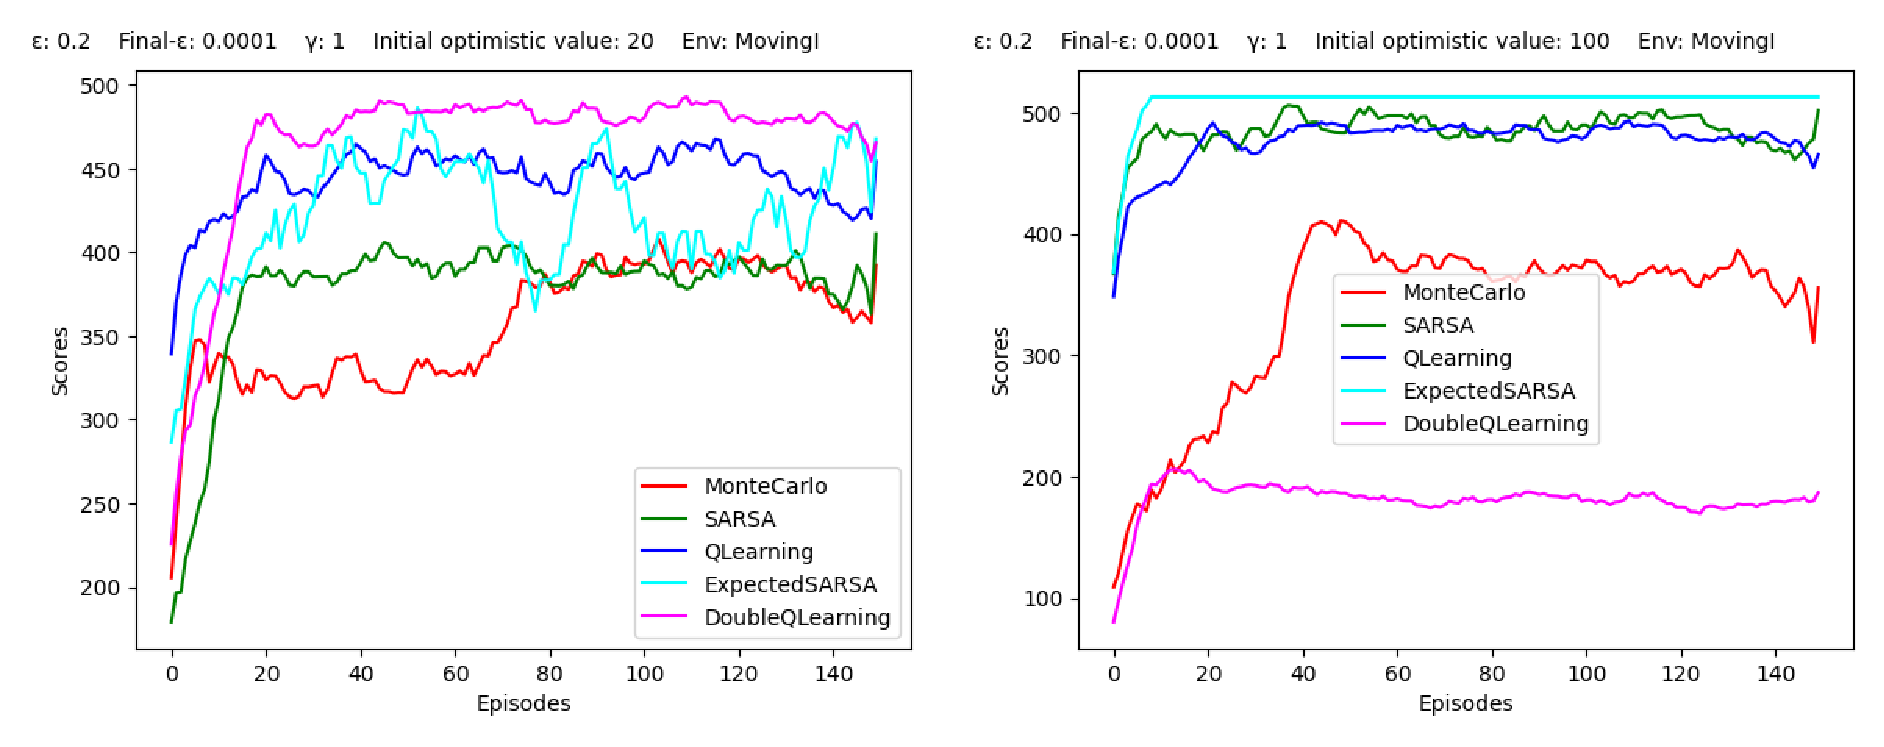
\includegraphics[width=\textwidth]{movingi}
    \caption{\texttt{MovingI} trap examples}
    \label{fig:movingi_eg}
\end{figure}

It is worth noting that there exist cases where the aforementioned variations in hyperparameter selection lead to highly desirable outcomes. This is exemplified by the results presented in Figures \ref{fig:i_eg} and \ref{fig:movingi_eg}, which demonstrate the efficacy of the \texttt{ExpectedSARSA} agent. Notably, on the right hand side of the both plots, the \texttt{ExpectedSARSA} agent was able to achieve optimal performance early on in the game with all seed values. \texttt{ExpectedSARSA} agent, in a very large number of experiments, has outperformed its counterparts, sometimes by a significant amount. This is particularly evident when considering its performance in simpler environments such as traps \texttt{I} and \texttt{MovingI}, where it is apparent that the agent is capable of learning extremely well. While other agents have performed well on these specific traps as well, their success may not be immediately apparent from the averaged results depicted in the plots.

Although performing these experiments with a larger number of seeds would ideally yield even more accurate results, we hope that the picture we presented provides a reasonable representation of the agents' performance in the demonstrated environments.

\section{Traps environment}
\begin{figure}[h]
    \centering
    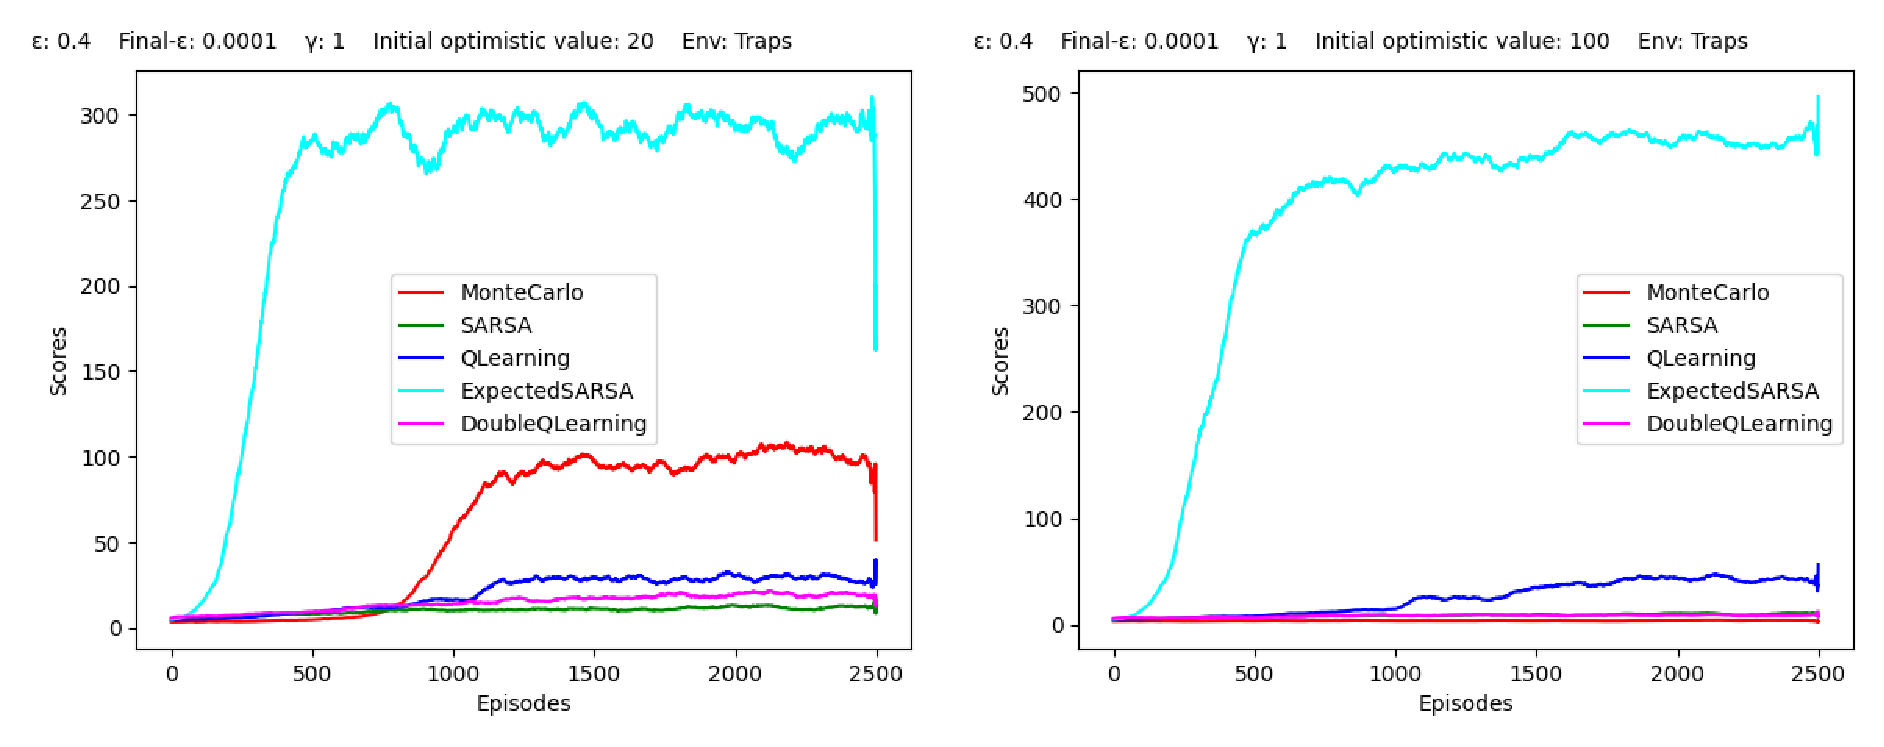
\includegraphics[width=\textwidth]{allTraps}
    \caption{All traps examples}
    \label{fig:alltraps_eg}
\end{figure}

This section delves into the exploration of a highly intricate environment of all traps combined, which is possibly the most complex one barring the full game. To clarify,\texttt{Traps} consist of all 10 individual traps mentioned in the previous section, and omit any bugs, virus or token type of obstacles. As depicted in Figure \ref{fig:alltraps_eg}, the majority of agents were unable to perform optimally in this environment. \texttt{ExpectedSARSA} was the only agent able to learn an optimal policy in any occurrence, as evidenced by its score nearing 500 in the right plot\footnote{It is worth mentioning that the plots for this environment have been smoothed with \texttt{window=100}.}, which was the approximate winning score value in all experiments. Moreover, \texttt{ExpectedSARSA} not only managed to learn an optimal policy once but did so with different hyperparameters and seed values on multiple occasions, leading to winning streaks of 30 games and early termination of the experiment. This outcome is the most favourable for any environment. The figure displays the averaged value of 9 seeds for all agents under the specified parameters. 

The experiments conducted for this environment were systematic and involved matching commonly used \texttt{eps} and \texttt{initOptVal} to test if the agents could learn. In these experiments, the difference in learning between the \texttt{ExpectedSARSA} agent and the others is even more pronounced. However, on the left plot visible in Figure \ref{fig:alltraps_eg}, and one instance, where \texttt{eps=0.4} and \texttt{initOptVal=20}, the \texttt{MonteCarlo} agent performed reasonably well, attaining an average score of approximately 100, which is substantially superior to the other agents, except for \texttt{ExpectedSARSA}.

\begin{figure}[h]
    \centering
    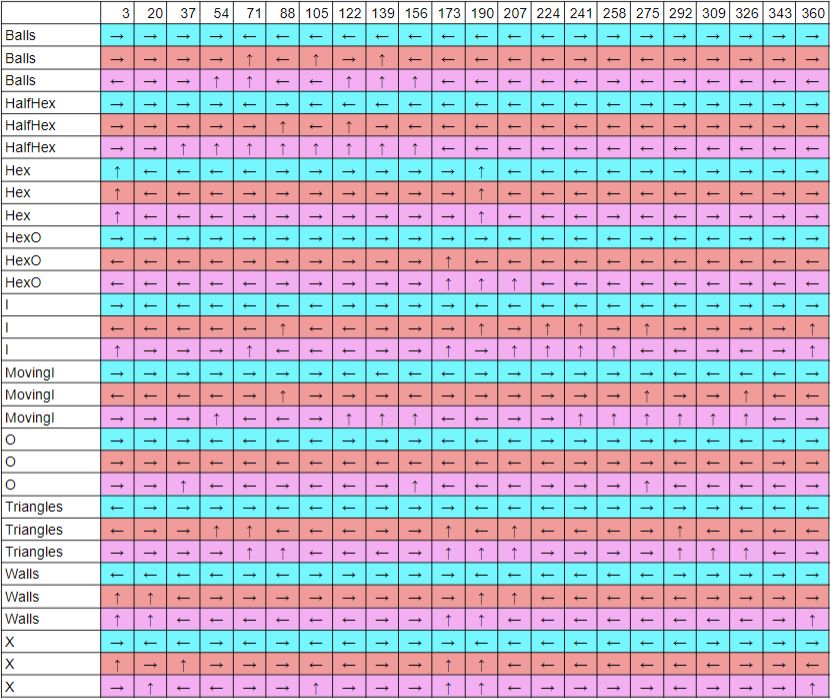
\includegraphics[width=0.8\textwidth]{allTraps_table}
    \caption{All traps with \texttt{ExpectedSARSA}, \texttt{MonteCarlo} and \texttt{DoubleQLearning} agents}
    \label{fig:traps_table_eg}
\end{figure}

When training in the all-traps environment I set the rots parameter to 22.  That's because it contains the Hex and Walls traps, which require a minimum of 22 rotations for learning to be feasible at all. This means that the number of states that with the individual trap environments corresponded to number of rotations, increased significantly. Considering that in this case we have 10 different trap types, there are 220 states with \texttt{Traps} environment. For that reason we picked \texttt{n=2500} for all of the experiments in this section. That's because in our experiments we've generally found that learning is most successful when the number of episodes is at least 10 times the number of states. Of course, it cannot be influenced by which states will be picked, since each game is generated randomly, but this was an estimation we used quite often during the experimentations. As a result of having this many \texttt{rots} values, with some simpler traps, there can be a lot of safe rotations that the agent can choose from. For that reason, going forward multiple adjacent states could be viable, if that particular trap requires for example \texttt{rots=6} when trained individually.

The content of the table in Figure \ref{fig:traps_table_eg} provides a comparison of policies from three different experiments, each reproduced with only one seed value, that yielded a satisfactory result. The purpose is to see how far off the agents were from an optimal policy. The blue rows represent the \texttt{ExpectedSARSA} agent, which performed with \texttt{eps=0.2} and \texttt{initOptVal=100}. The agent stopped an experiment early, after 437 games with initial number of games (\texttt{n}) being 2500. Considering it won 30 games in a row, each one lasting 15 levels, we can assume, with high probability, the learned policy is optimal for this environment. The red rows represent the \texttt{MonteCarlo} agent, which performed reasonably well with \texttt{eps=0.2} and \texttt{initOptVal=20}, winning 282/2500 games, but the experiment did not terminate early, suggesting a suboptimal policy. The pink rows represents the \texttt{QLearning} agent, which won 142/2500 games with \texttt{eps=0.4} and \texttt{initOptVal=20}. It should be noted that the combination of a seed value and hyperparameters that yielded the best results were picked for the \texttt{MonteCarlo} and \texttt{QLearning} agents, and in other cases, they won fewer or no games under this environment. Lastly it should be noted that, \texttt{SARSA(S)} and \texttt{DoubleQLearning}  performed poorly, with average scores in all experiments under all hyper parameter combinations, being not more than 20.

Multiple instances in the data show the phenomenon discussed in Section \ref{intbeh} of this chapter. For instance, upon closer examination of rotation values 54 and 71 in the rows pertaining to the Balls trap, it becomes evident that the \texttt{ExpectedSARSA} agent opted to alternate between those two rotation types, whereas the other two agents, \texttt{Monte Carlo} and \texttt{QLearning}, chose to proceed using only one or both of the rotations. This trend can be observed in several other cases within the data, and it is highly probable that, with so many rotation options available, any of the three methods would lead to the agent safely passing the trap. Nevertheless, it is a fact that \texttt{ExpectedSARSA} learned a better policy than \texttt{MonteCarlo} and \texttt{QLearning}. However, for certain traps, all or at least two of the agents had satisfactory policies (such as the \texttt{Hex} trap), whereas for others, \texttt{MonteCarlo} and/or \texttt{QLearning} were observed taking actions that could not be deemed optimal when compared to the \texttt{ExpectedSARSA} agent. An example of such an instance can be found in rotation values 275 and 292 with trap \texttt{X}, where the \texttt{QLearning} agent attempted to switch between the two rotations to pass, while both \texttt{ExpectedSARSA} and \texttt{MonteCarlo} avoided it, suggesting that remaining in that rotation was not safe and that the agent should try to move to another rotation in a timely manner.

\section{Tokens environment}
\begin{figure}[h]
    \centering
    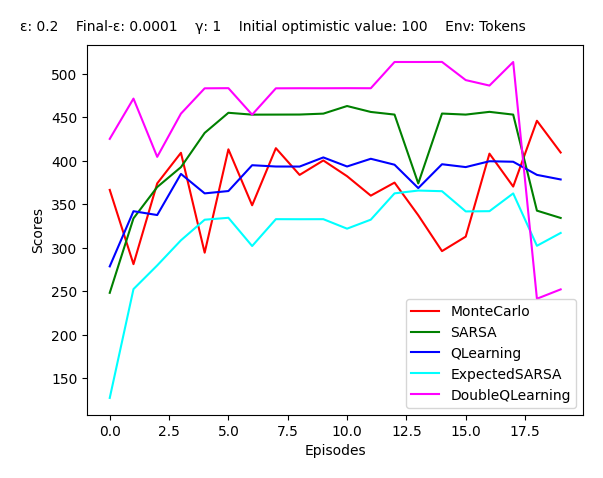
\includegraphics[width=0.6\textwidth]{tokensEnv}
    \caption{\texttt{Tokens} example}
    \label{fig:tokens}
\end{figure}

The Tokens environment is characterized by its simplicity, as it lacks obstacles that pose a lethal threat to the agent. The agent's task is to collect tokens at regular intervals to prevent its battery from draining completely. The number of rotations needed in this environment is six, making it relatively easy to train. Figure \ref{fig:tokens} illustrates that the average performance of all agents is commendable, even when \texttt{n=20}\footnote{Note that smoothing was applied to this plot.}. In subsequent sections, we will delve into more intriguing findings when tokens are incorporated into a larger environment, and explore their impact on the behaviour of the agents.

\section{Individual Bugs and Viruses environments}
\begin{figure}[h]
    \centering
    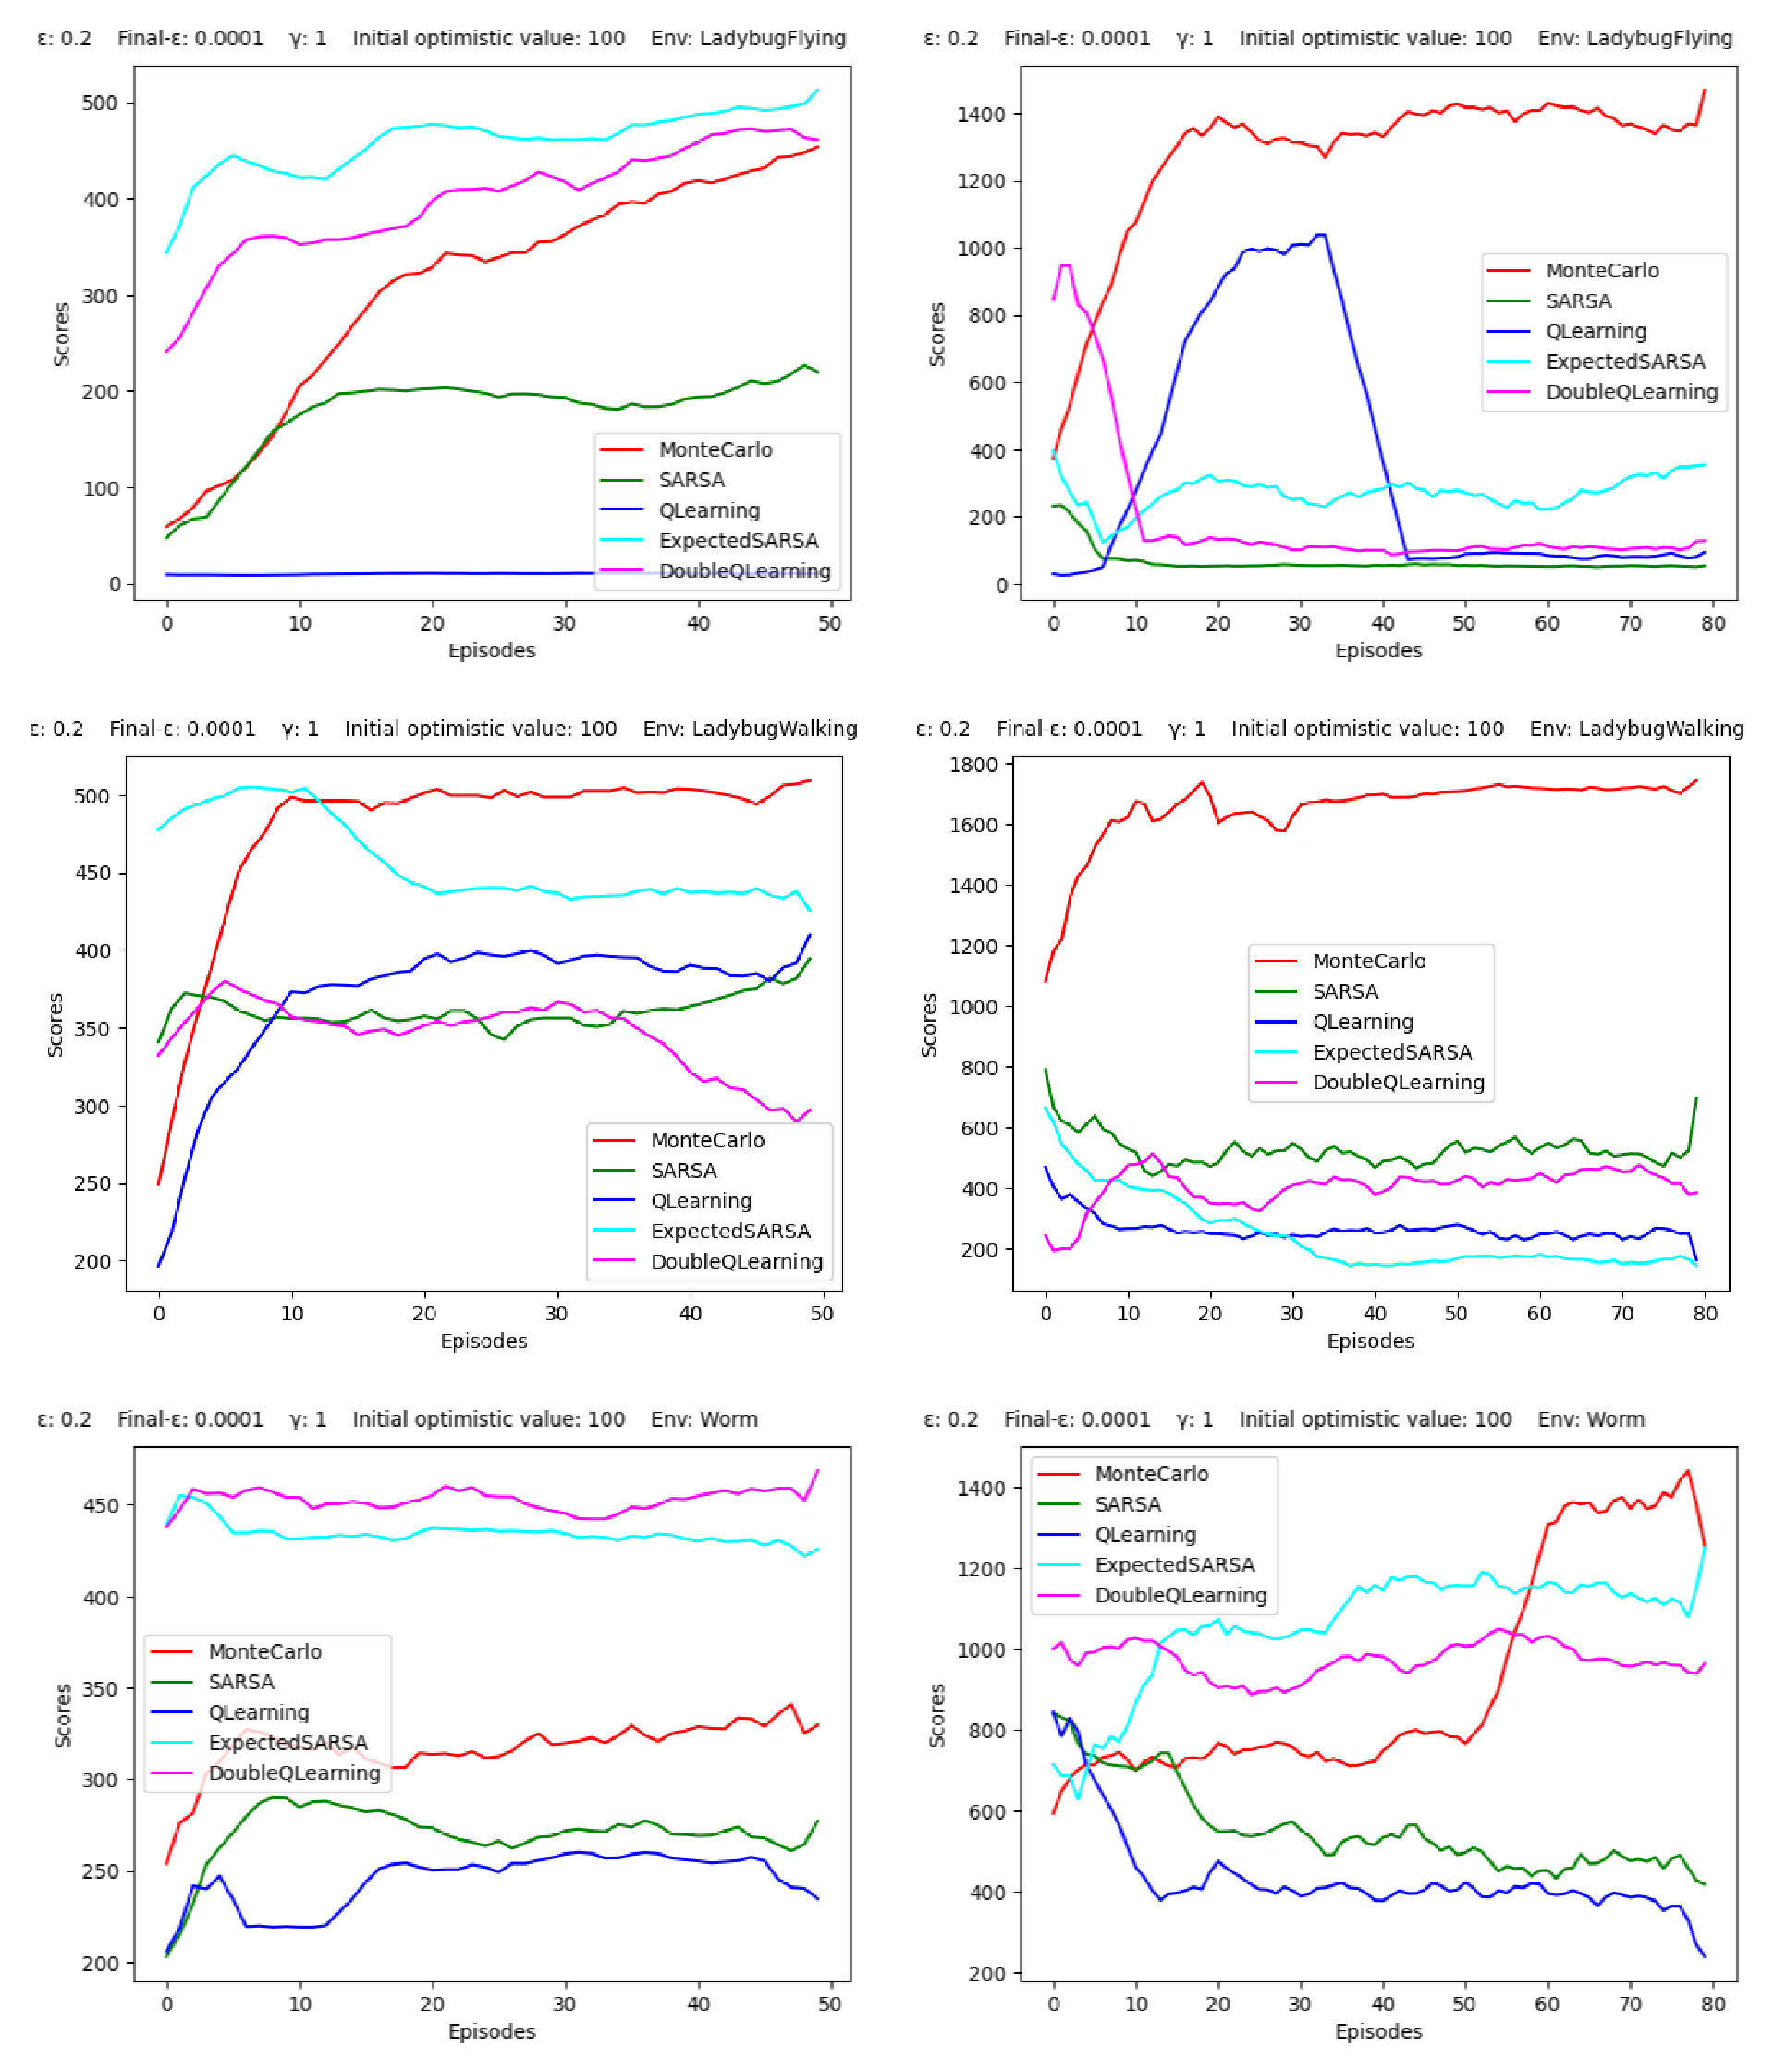
\includegraphics[width=0.9\textwidth]{bugs_ind}
    \caption{\texttt{LadybugFlying}, \texttt{LadybugWalking} and \texttt{Worm} environments examples}
    \label{fig:bugs_ind_eg}
\end{figure}

In this section, we aim to investigate two types of environments that have not been discussed before: Bugs and Viruses. These environments include three (\texttt{Worm, LadibugWalkingm LadybugFlying}) and two (\texttt{Bacteriophage, Rotavirus}) obstacles, respectively, and are different from environments that consist solely of trap-type obstacles. One key difference is that the agent can also use its ability to shoot in \texttt{Bugs} and \texttt{Viruses} environments. This means that, for the first time in this chapter, our agents have 6 actions to choose from, and we aim to analyse how this affects their behaviour.

We begin by showcasing the performance of all agents on individual bugs or viruses. For this purpose, we have evaluated their performance on 50 games, each with \texttt{eps=0.2} and \texttt{initialOptVal=100.0}. We chose these parameters as they resulted in the best overall performance of the agents. The plots presenting all agents in this section are an average of five different seeds, and each plot has been smoothed with a \texttt{window=10}. The left-hand side of both figures displays the agents' performance when shooting was not enabled, whereas the right-hand side depicts the scores when the agents could shoot.

\begin{figure}[h]
    \centering
    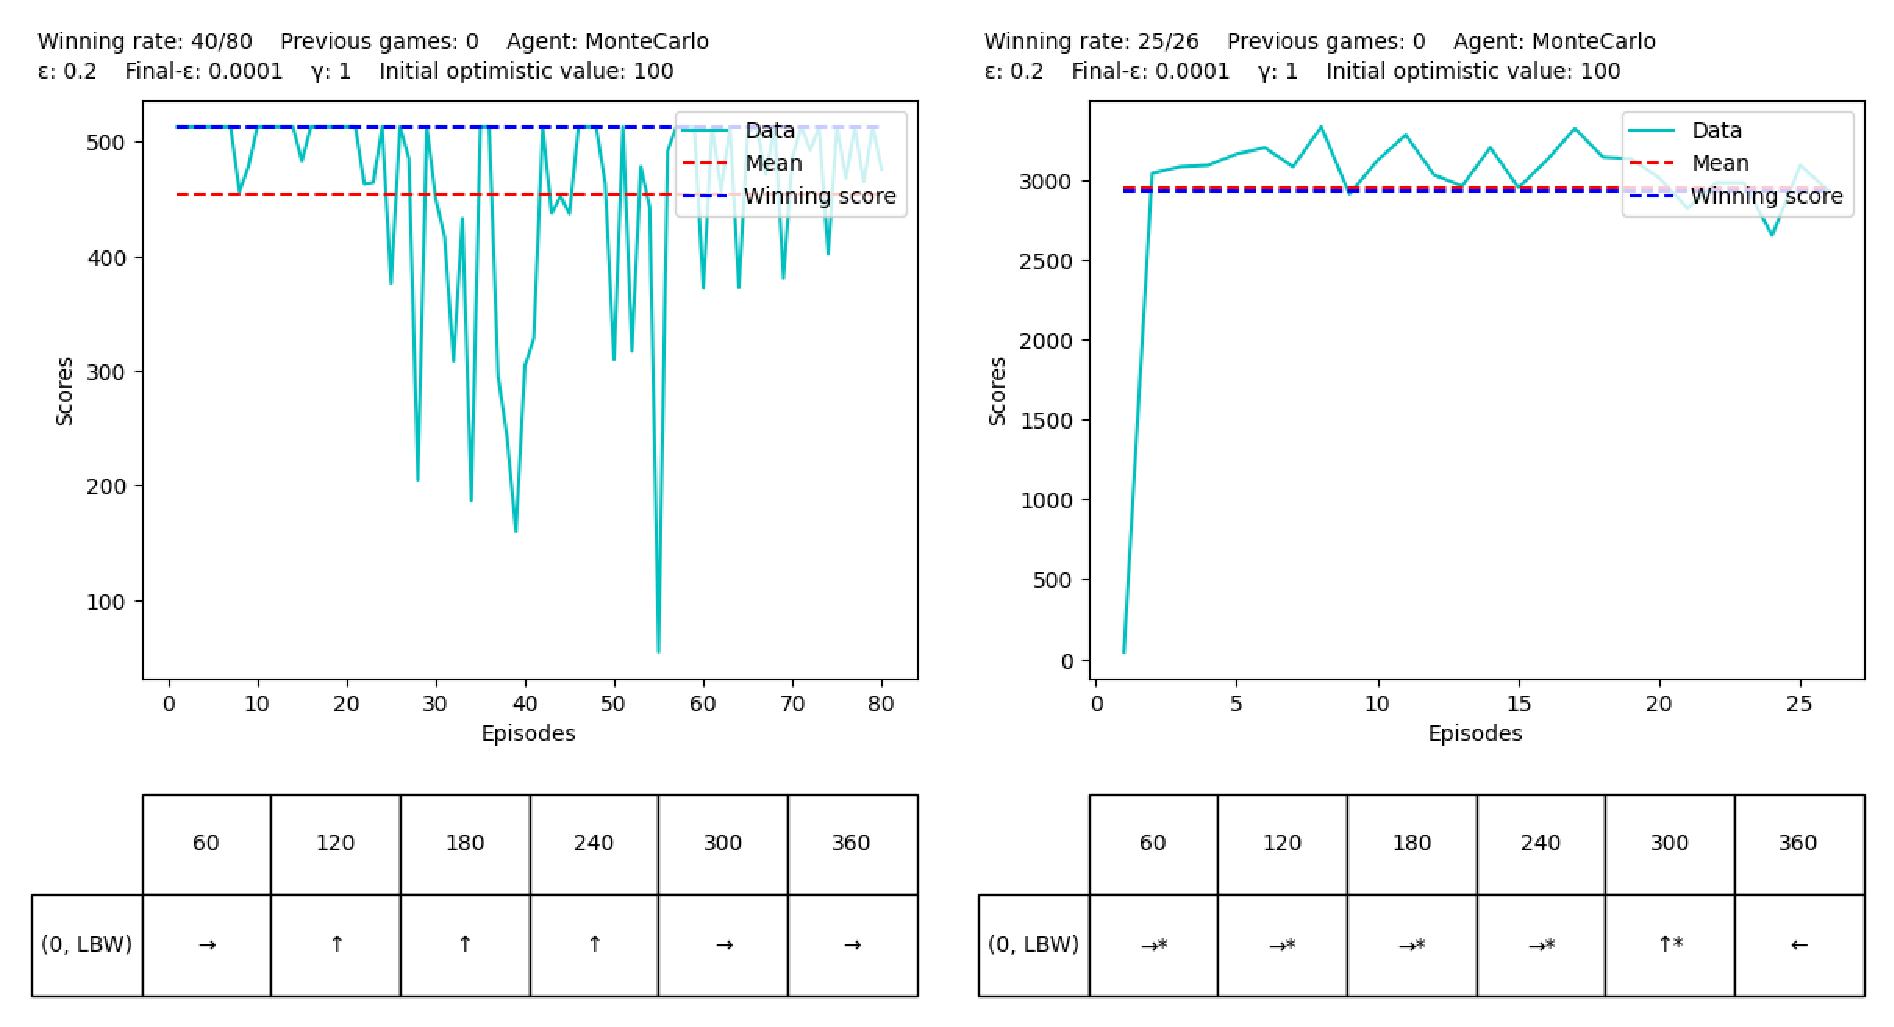
\includegraphics[width=0.8\textwidth]{bugs_ind_mc}
    \caption{\texttt{LadybugWalking} with \texttt{MonteCarlo} agent examples}
    \label{fig:bugs_ind_mc_eg}
\end{figure}

The category of obstacles referred to as bugs in the game environment behaves differently from viruses or traps. This is due to the fact that Hans, only loses energy upon contact with any of the bug type obstacles, and only when the battery life is depleted to 0\% does the game terminate, or when the game is won. The performance of some agents in this environment is lower than in others, as illustrated in Figure \ref{fig:bugs_ind_eg}. However, the \texttt{MonteCarlo} agent consistently performs well, particularly with the \texttt{LadybugWalking} obstacle. Conversely, the \texttt{QLearning} agent appears to perform poorly in this environment, suggesting that it may not be the most suitable method for these seemingly inconsistent bug obstacles. As battery life is not part of the state value, the ideal behaviour for the agent would be to either always shoot (if permitted) or always avoid the these obstacles. This behaviour is precisely what is observed in Figure \ref{fig:bugs_ind_mc_eg}, where the \texttt{MonteCarlo} agent does not shoot at all in the left plot (suggesting that its avoiding the obstacles), while in the right one, it shoots in almost all actions. Although the left plot may not have achieved an optimal policy, it has derived one that allows the agent to win at least 50\% of the time.

\begin{figure}[h]
    \centering
    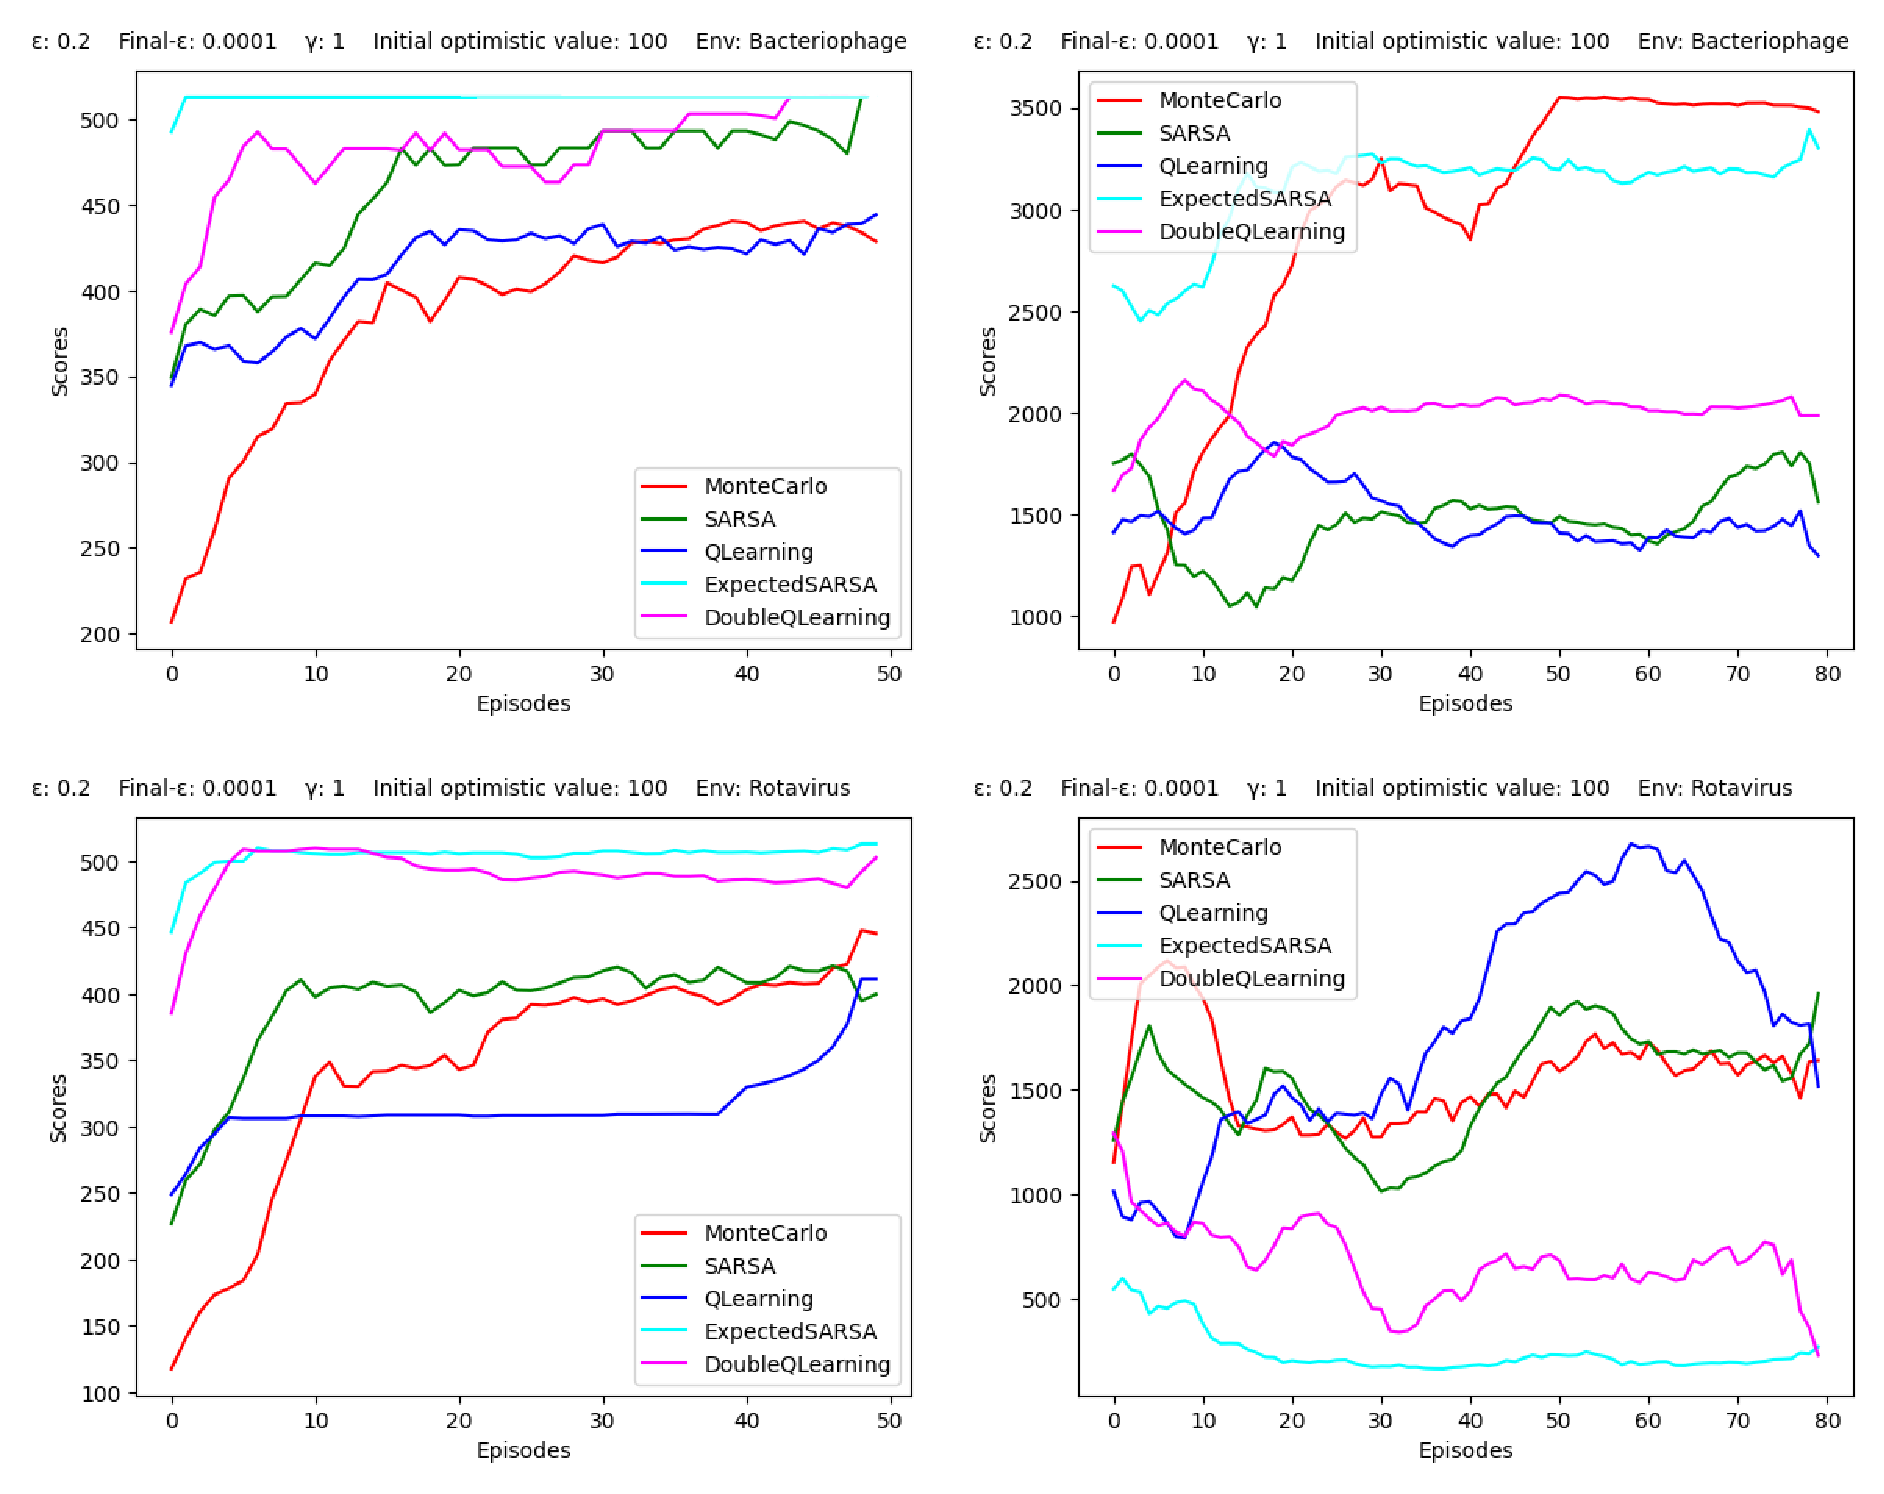
\includegraphics[width=0.8\textwidth]{viruses_ind}
    \caption{\texttt{Bacteriophage} and \texttt{Rotavirus} environments examples}
    \label{fig:viruses_ind_eg}
\end{figure}

Figure \ref{fig:viruses_ind_eg} displays the performance of the agents for each virus type obstacle. Notably, \texttt{ExpectedSARSA} exhibited a high level of performance in both cases where shooting was not enabled. However, in the case of \texttt{Rotavirus} when the shooting was involved, it performed the worst out of all the agents. It is possible that the agent was confused by the\texttt{Rotavirus} behaviour, since when Hans hits a \texttt{Rotavirus} for the first time, he becomes sick, and if it is hit again during his sick period, it results in his death. In contrast, the behaviour of \texttt{Bacteriophage} is more akin to the traps, as it kills Hans on the spot upon contact.

\begin{figure}[h]
    \centering
    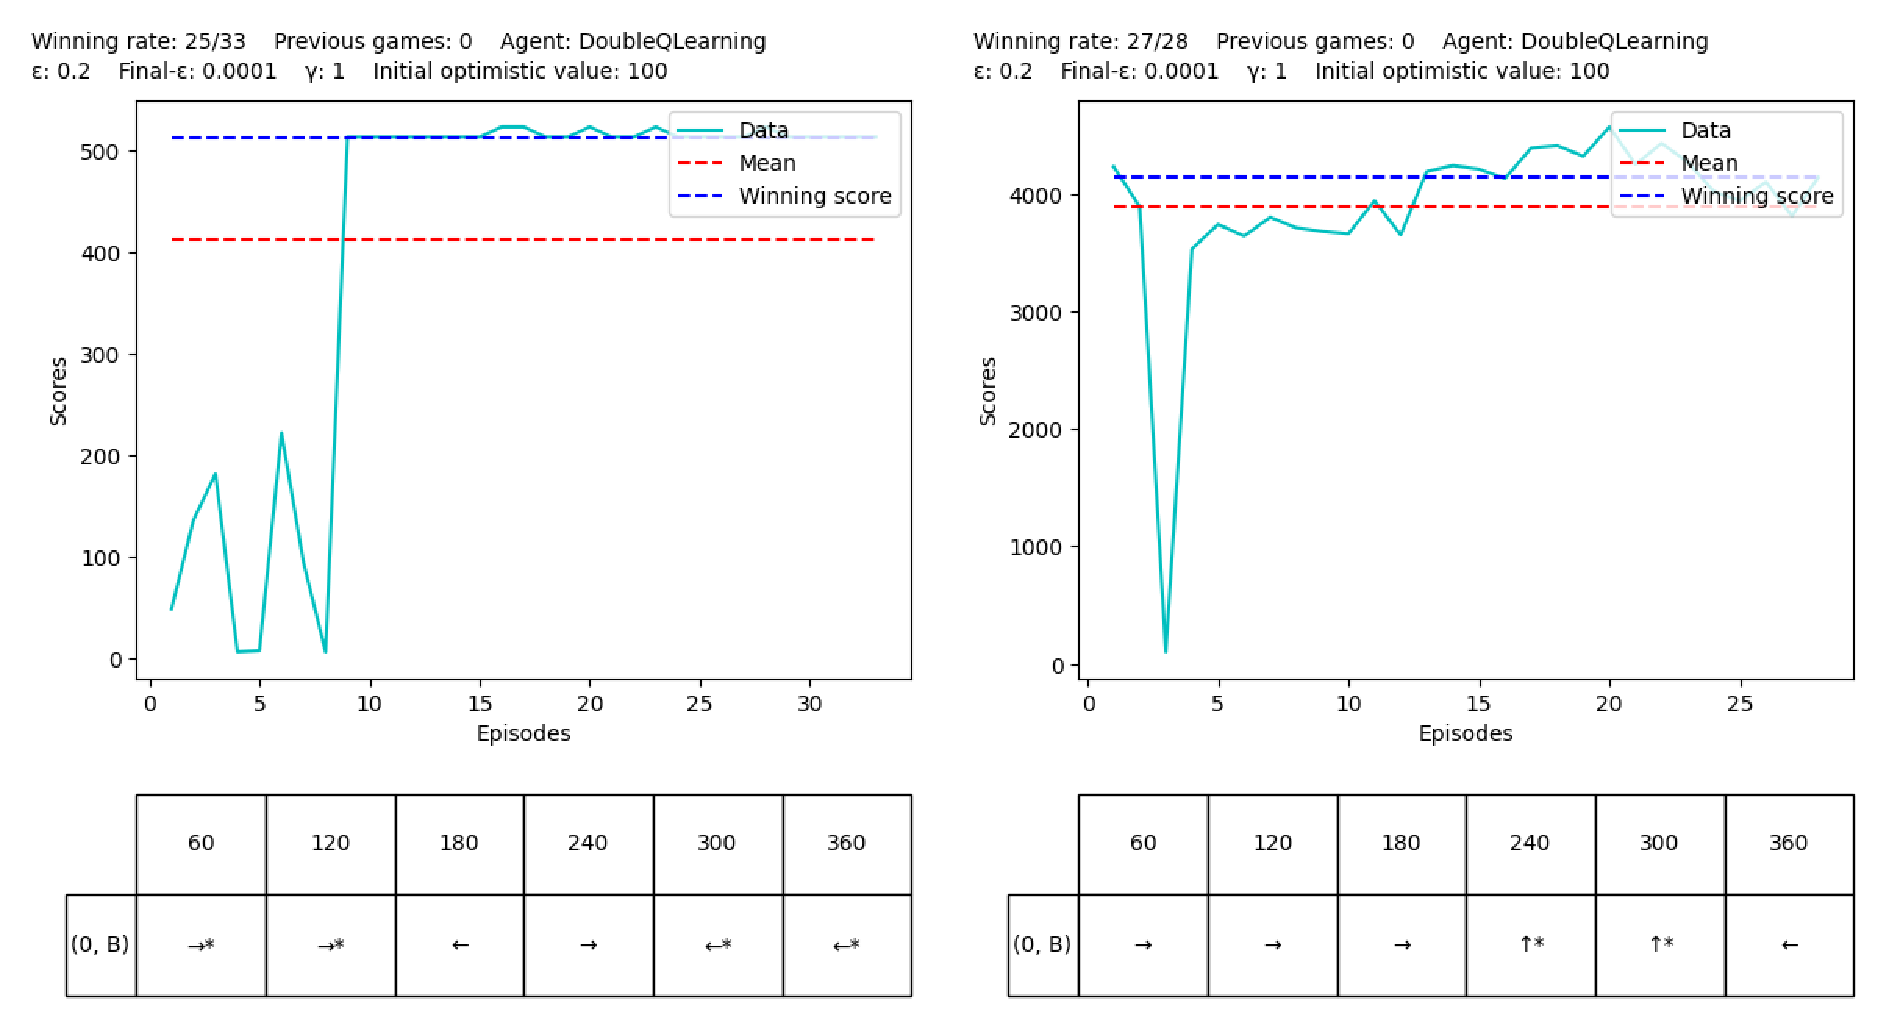
\includegraphics[width=0.8\textwidth]{viruses_ind_dql}
    \caption{\texttt{Rotavirus} environment with \texttt{DoubleQLearning} agent examples}
    \label{fig:viruses_ind_dql_eg}
\end{figure}

To diverge a little from the performance of the agents all together, lets take a look into Figure \ref{fig:viruses_ind_dql_eg} which shows two instances of the \texttt{DoubleQLearning} agent with the \texttt{Rotavirus} obstacle and \texttt{shooting=enabled}. Each plot used only one seed value and the smoothing was not applied. In both of the cases in this figure, the agent learned an optimal policy and thus terminated the game early. However, for the left plot, even though there are some actions in which the agent chooses to shoot, it doesn't actually shoot down any obstacles. This is evident by the fact that the winning score is only around 500, which is the minimum winning score achieved after 15 levels.  This might explain why in these conditions, the \texttt{DoubleQLearning} agent did not perform as well as some of the others in the overall performance analysis (Figure \ref{fig:viruses_ind_eg}). On the other hand, the right plot shows a policy in which that the agent learned to shoot down the \texttt{Rotavirus} obstacles and achieved a much higher winning score, demonstrating the importance of properly utilizing the shooting action when it is enabled.

\section{Bugs and Viruses environments}
\begin{figure}[h]
    \centering
    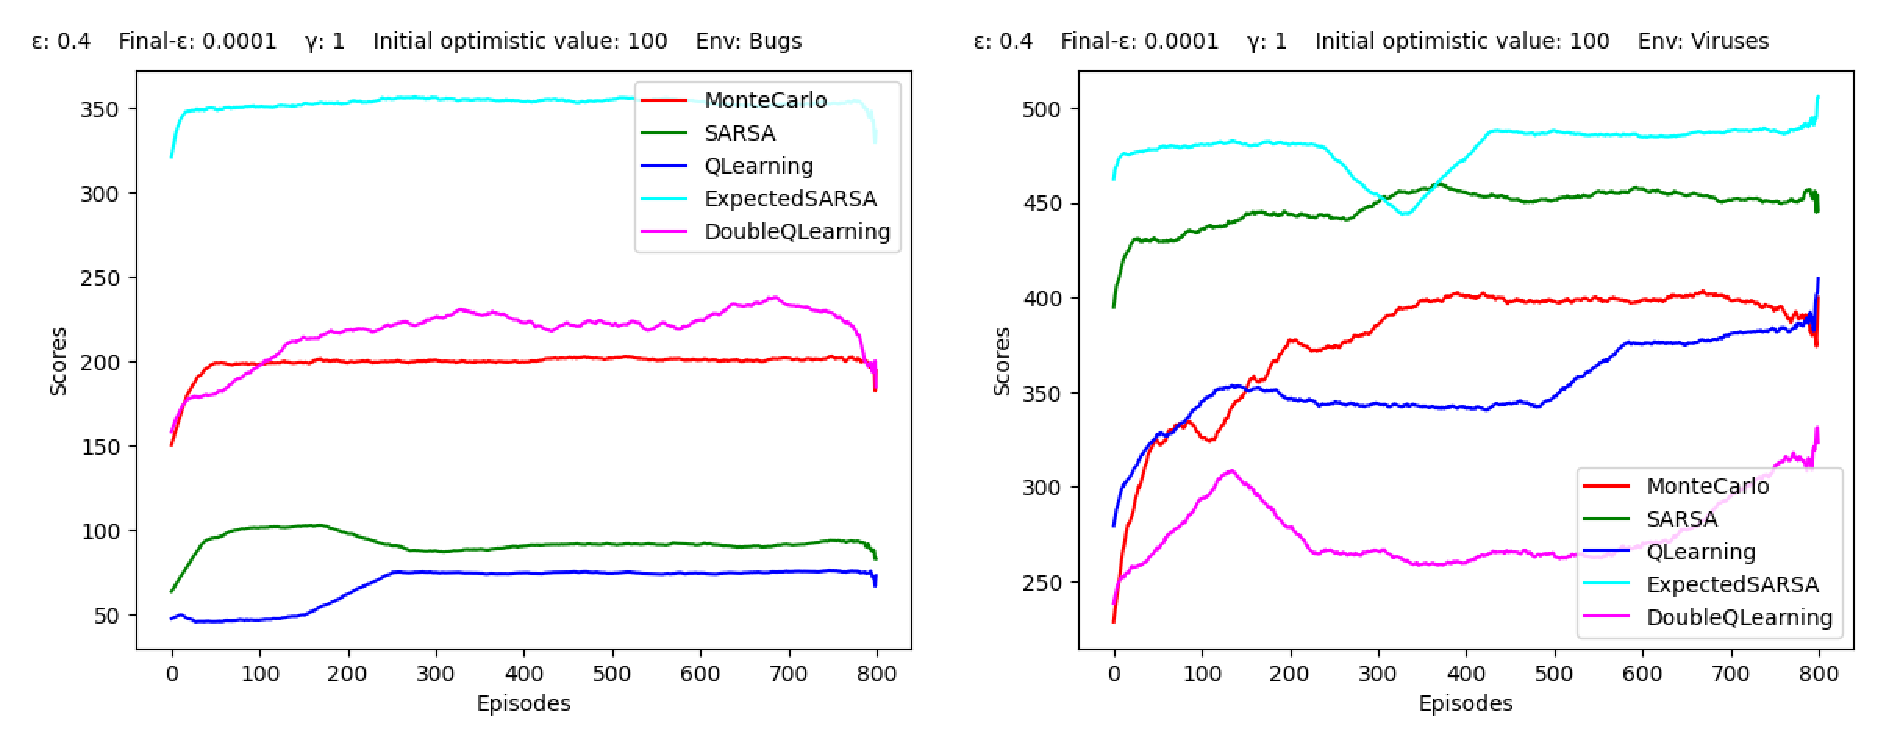
\includegraphics[width=0.9\textwidth]{BV800ns}
    \caption{\texttt{Bugs} and \texttt{Viruses} environments examples}
    \label{fig:bv800ns_eg}
\end{figure}

The current section compares the performance of agents in the full \texttt{Bugs} or \texttt{Viruses} environments and their combination with \texttt{Tokens} when faced with the same hyperparameters. Plots that display the performance of all agents in this section are averaged over 10 seeds and smoothed with \texttt{window=100}. In Figure \ref{fig:bv800ns_eg} we see the average performance of the agents when shooting is not allowed. Similar to the traps environment, the \texttt{ExpectedSARSA} agent exhibited the best performance. On the other hand, when faced with the full \texttt{Bugs} environment, \texttt{QLearning} agent showed similar behaviour to that seen on individual bugs obstacles and performed worse than the other agents.

\begin{figure}[h]
    \centering
    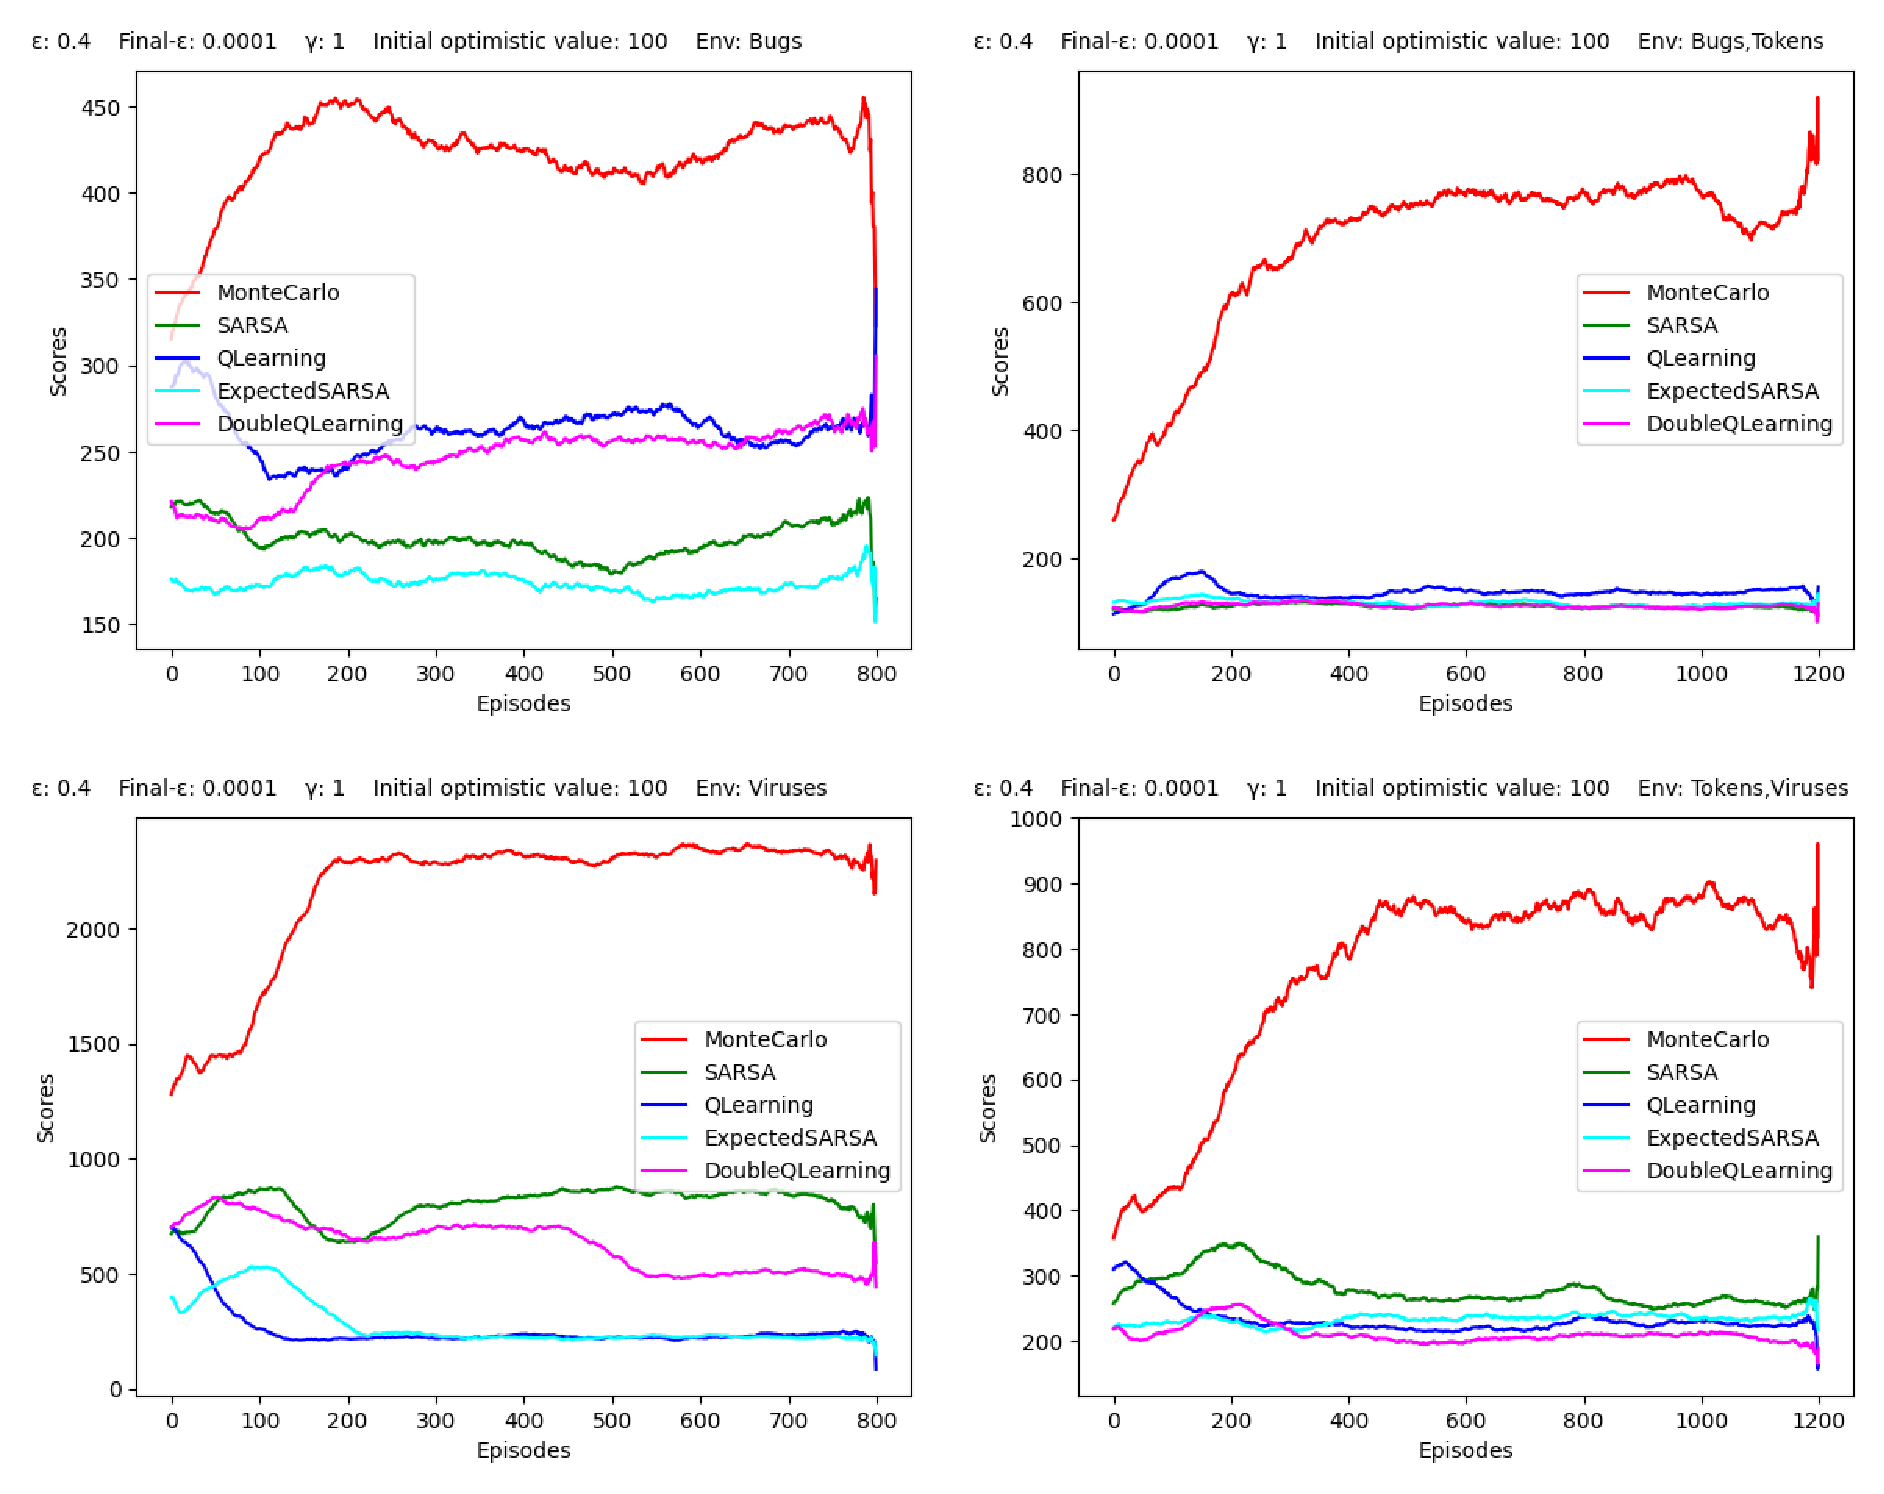
\includegraphics[width=0.8\textwidth]{bbt_vvt}
    \caption{\texttt{Bugs},\texttt{Viruses} and their combination with \texttt{Tokens} examples}
    \label{fig:bbt_vvt_eg}
\end{figure}

Figure \ref{fig:bbt_vvt_eg} shows plots where shooting actions are available to the agent. Here, the \texttt{MonteCarlo} agent had the best performance in all four cases. An interesting result is that when faced with \texttt{env=[Bugs,Tokens]}, this agent performed better than in the only \texttt{Bugs} environment, while with \texttt{env=[Viruses,Tokens]}, it performed worse than with \texttt{Viruses} alone. Considering how running into a bug influences Hans, adding \texttt{Tokens} to the \texttt{Bugs} environment was beneficial as long as the tokens were picked up when possible and the agent was conservative with shooting. In contrast, in the environment containing both \texttt{Viruses} and \texttt{Tokens}, the agent could still easily lose if Hans rans into \texttt{Bacteriophage} once or \texttt{Rotavirus} twice in a row. When having unlimited shooting in \texttt{Viruses} environment alone, all agents performed much better than when \texttt{Tokens} were part of it as well.

Overall, in environments that combine Tokens, the ratio of shooting and no shooting actions was approximately even. 

\begin{figure}[h]
    \centering
    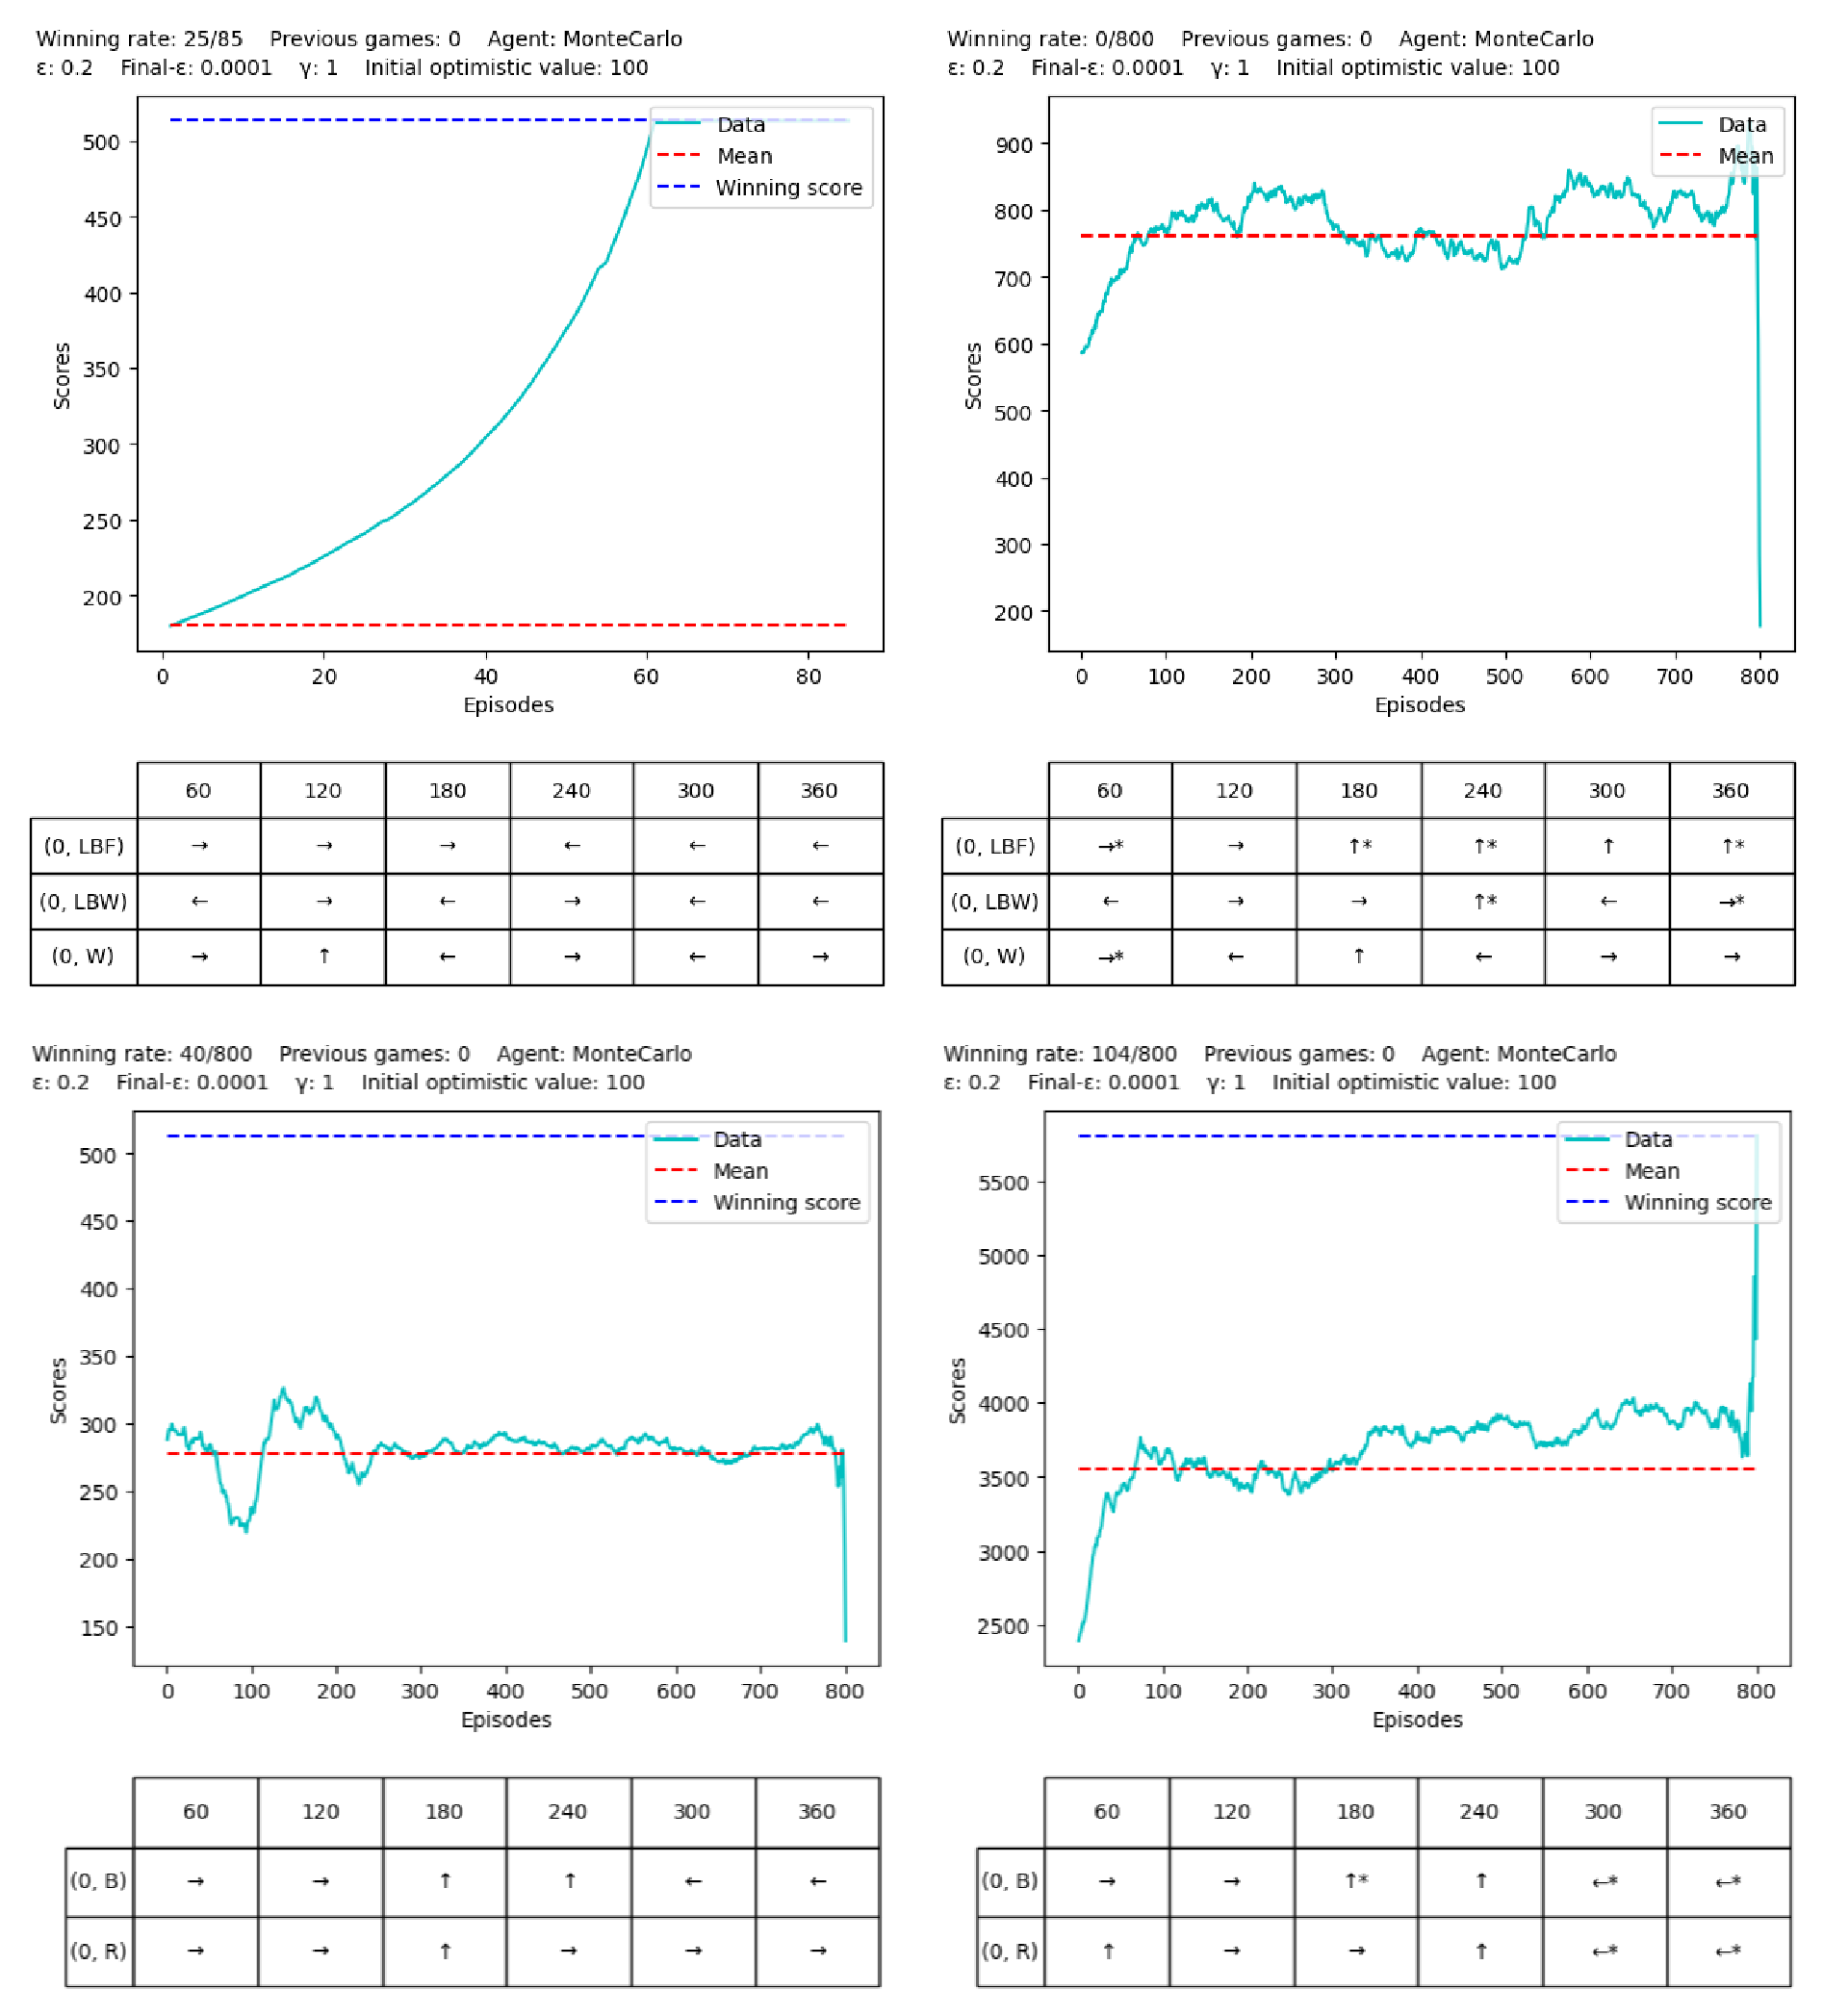
\includegraphics[width=\textwidth]{BV_02_100_1}
    \caption{\texttt{Bugs} and \texttt{Viruses} with and without shooting comparison}
    \label{fig:BV_02_100_1_eg}
\end{figure}


In Figure \ref{fig:BV_02_100_1_eg}, the performance of \texttt{MonteCarlo} agent shown environments is displayed for specific hyperparameters and with the same seed value (smoothing window value is 100). For each environment, two plots were created, one where the agent is allowed to shoot and another where shooting is disabled. The two plots depicting \texttt{Bugs} exhibit noticeable differences, as the agent found an optimal policy when shooting was not available. With shooting enabled, even though the direction of the agent's movement for each state is quite similar to the ones in the first plot, it failed to win any games. In contrast, with the \texttt{Viruses} environment, the agent's movement is almost identical in both cases, and the plot shows that the agent performed similarly well, with the right plot showing an average and winning scores approximately 10 times higher than on the left, as a consequence of the ability to shoot and due to that gain higher scores.

\section{Full game environment}
In this section, we explore the performance of the agents in the most challenging environment, full game. The results of these experiments are not surprising, given the complexity of the environment. In the figures presented in this section, we averaged the results of 10 seeds, and each plot was smoothed with a window of 100. The left side of the plots shows the performance of the agents in the environment where shooting is disabled, while the right side shows the environment where shooting is enabled. The right side was trained on 2000 more games than the left one considering that the number of actions possible increased.

\begin{figure}[h]
    \centering
    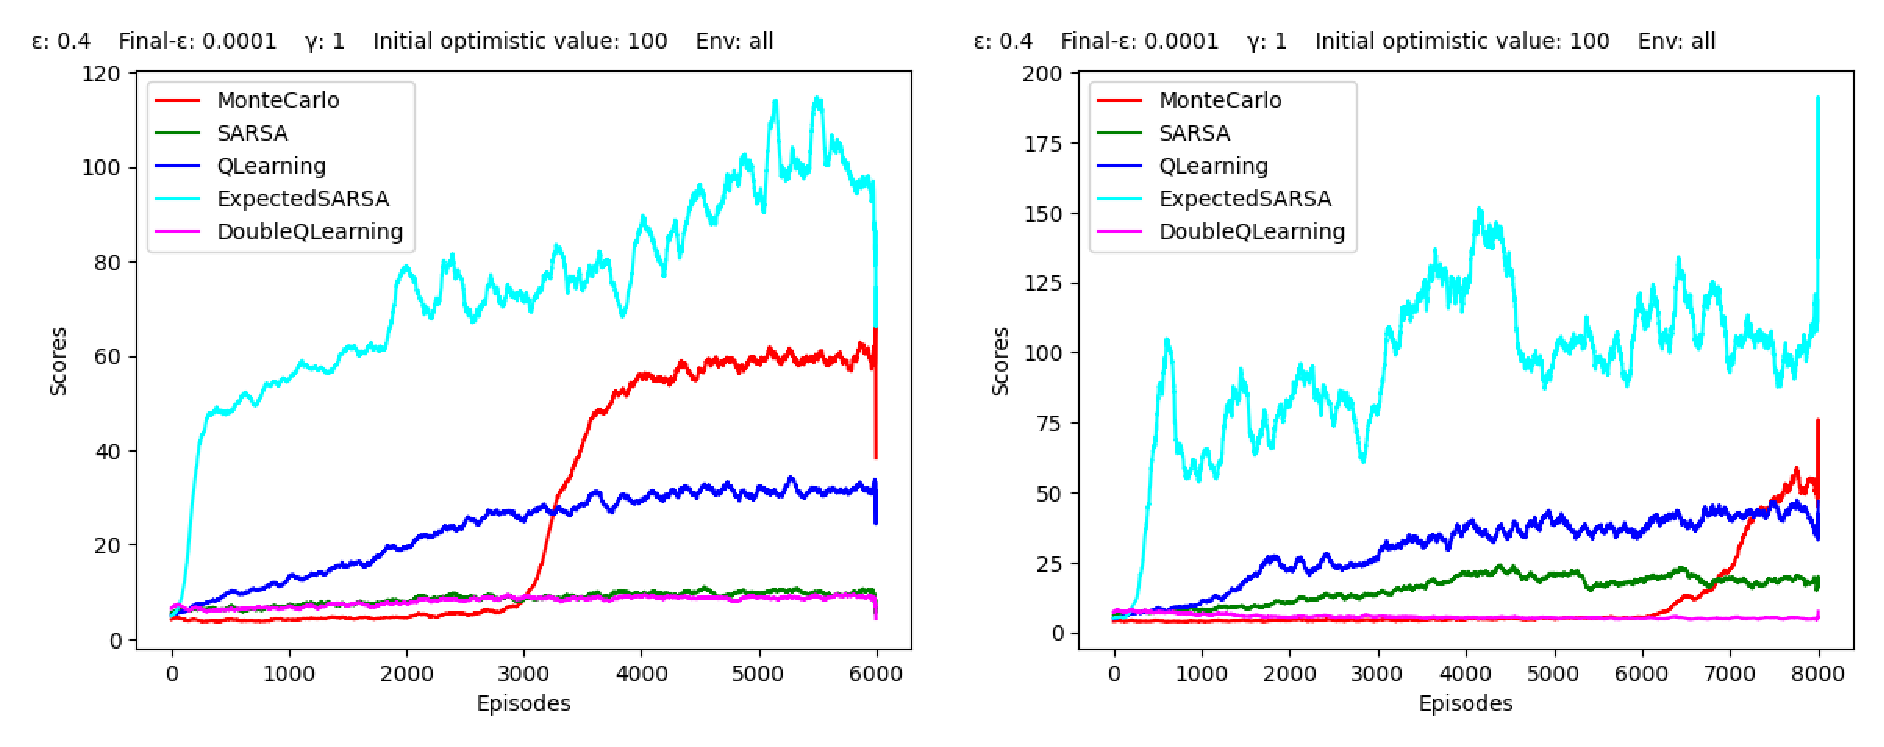
\includegraphics[width=\textwidth]{full_game}
    \caption{Full game example}
    \label{fig:full_game_eg}
\end{figure}

Looking at Figure 1, we can see that in the environment without shooting, ExpectedSARSA performed the best, as expected. The scores of MonteCarlo and QLearning agents were not too bad, considering the complexity of the environment and the fact that QLearning agent underperformed in the Bugs environment. On the right plot, ExpectedSARSA is still in the lead compared to the other agents. However, considering that the agents were allowed to shoot in this case, the scores did not improve significantly.

\begin{figure}[h]
    \centering
    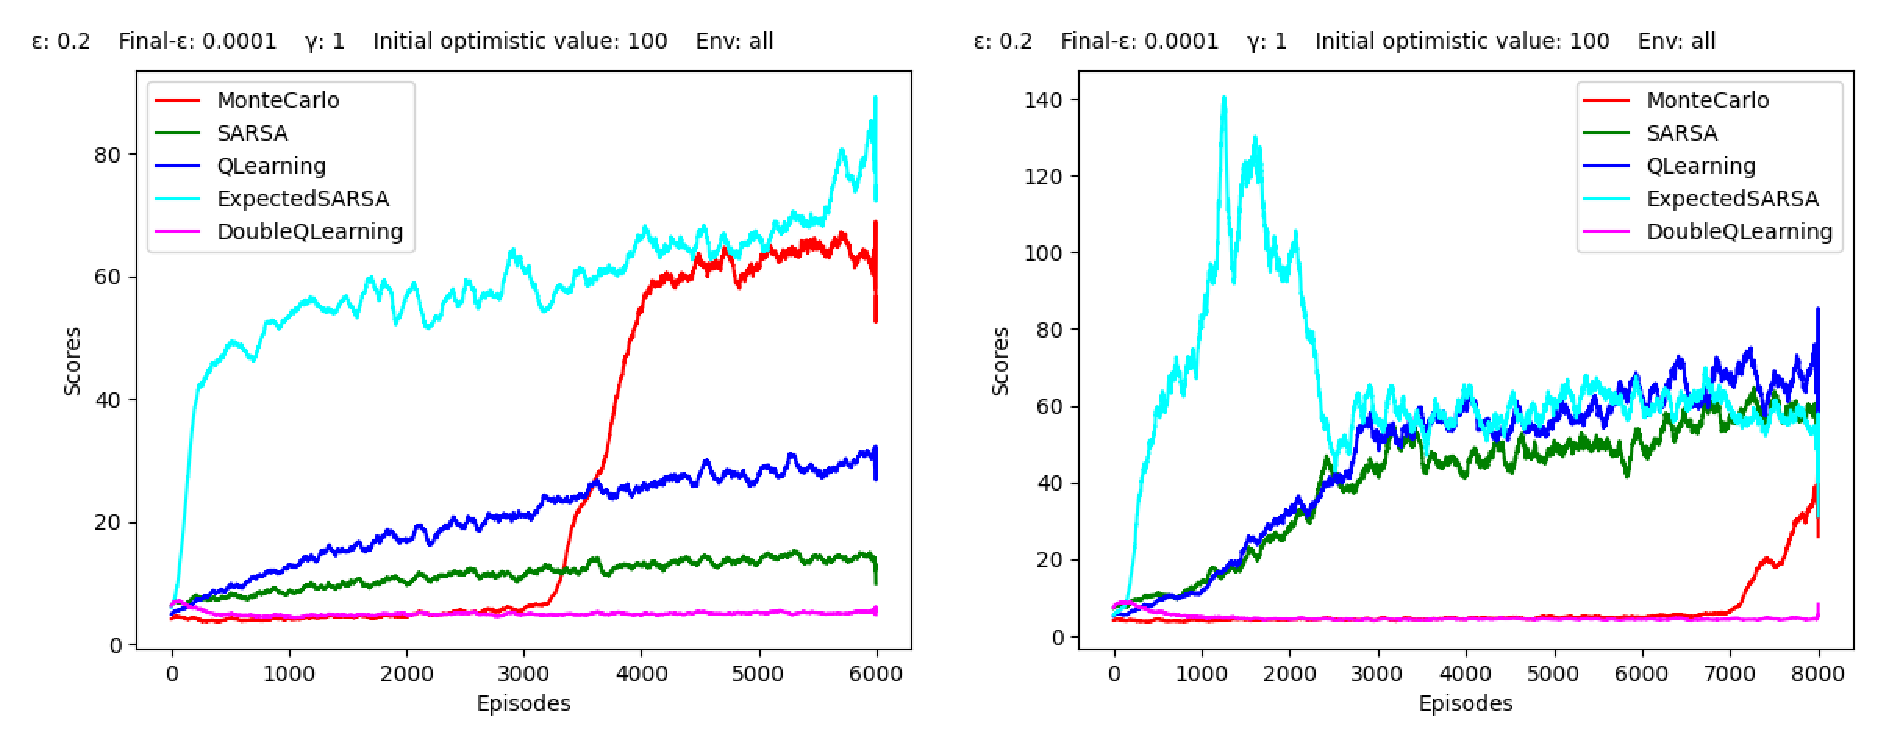
\includegraphics[width=\textwidth]{full_game_cf}
    \caption{Catastrophic forgetting example}
    \label{fig:full_game_cf_eg}
\end{figure}
\begin{figure}[h]
    \centering
    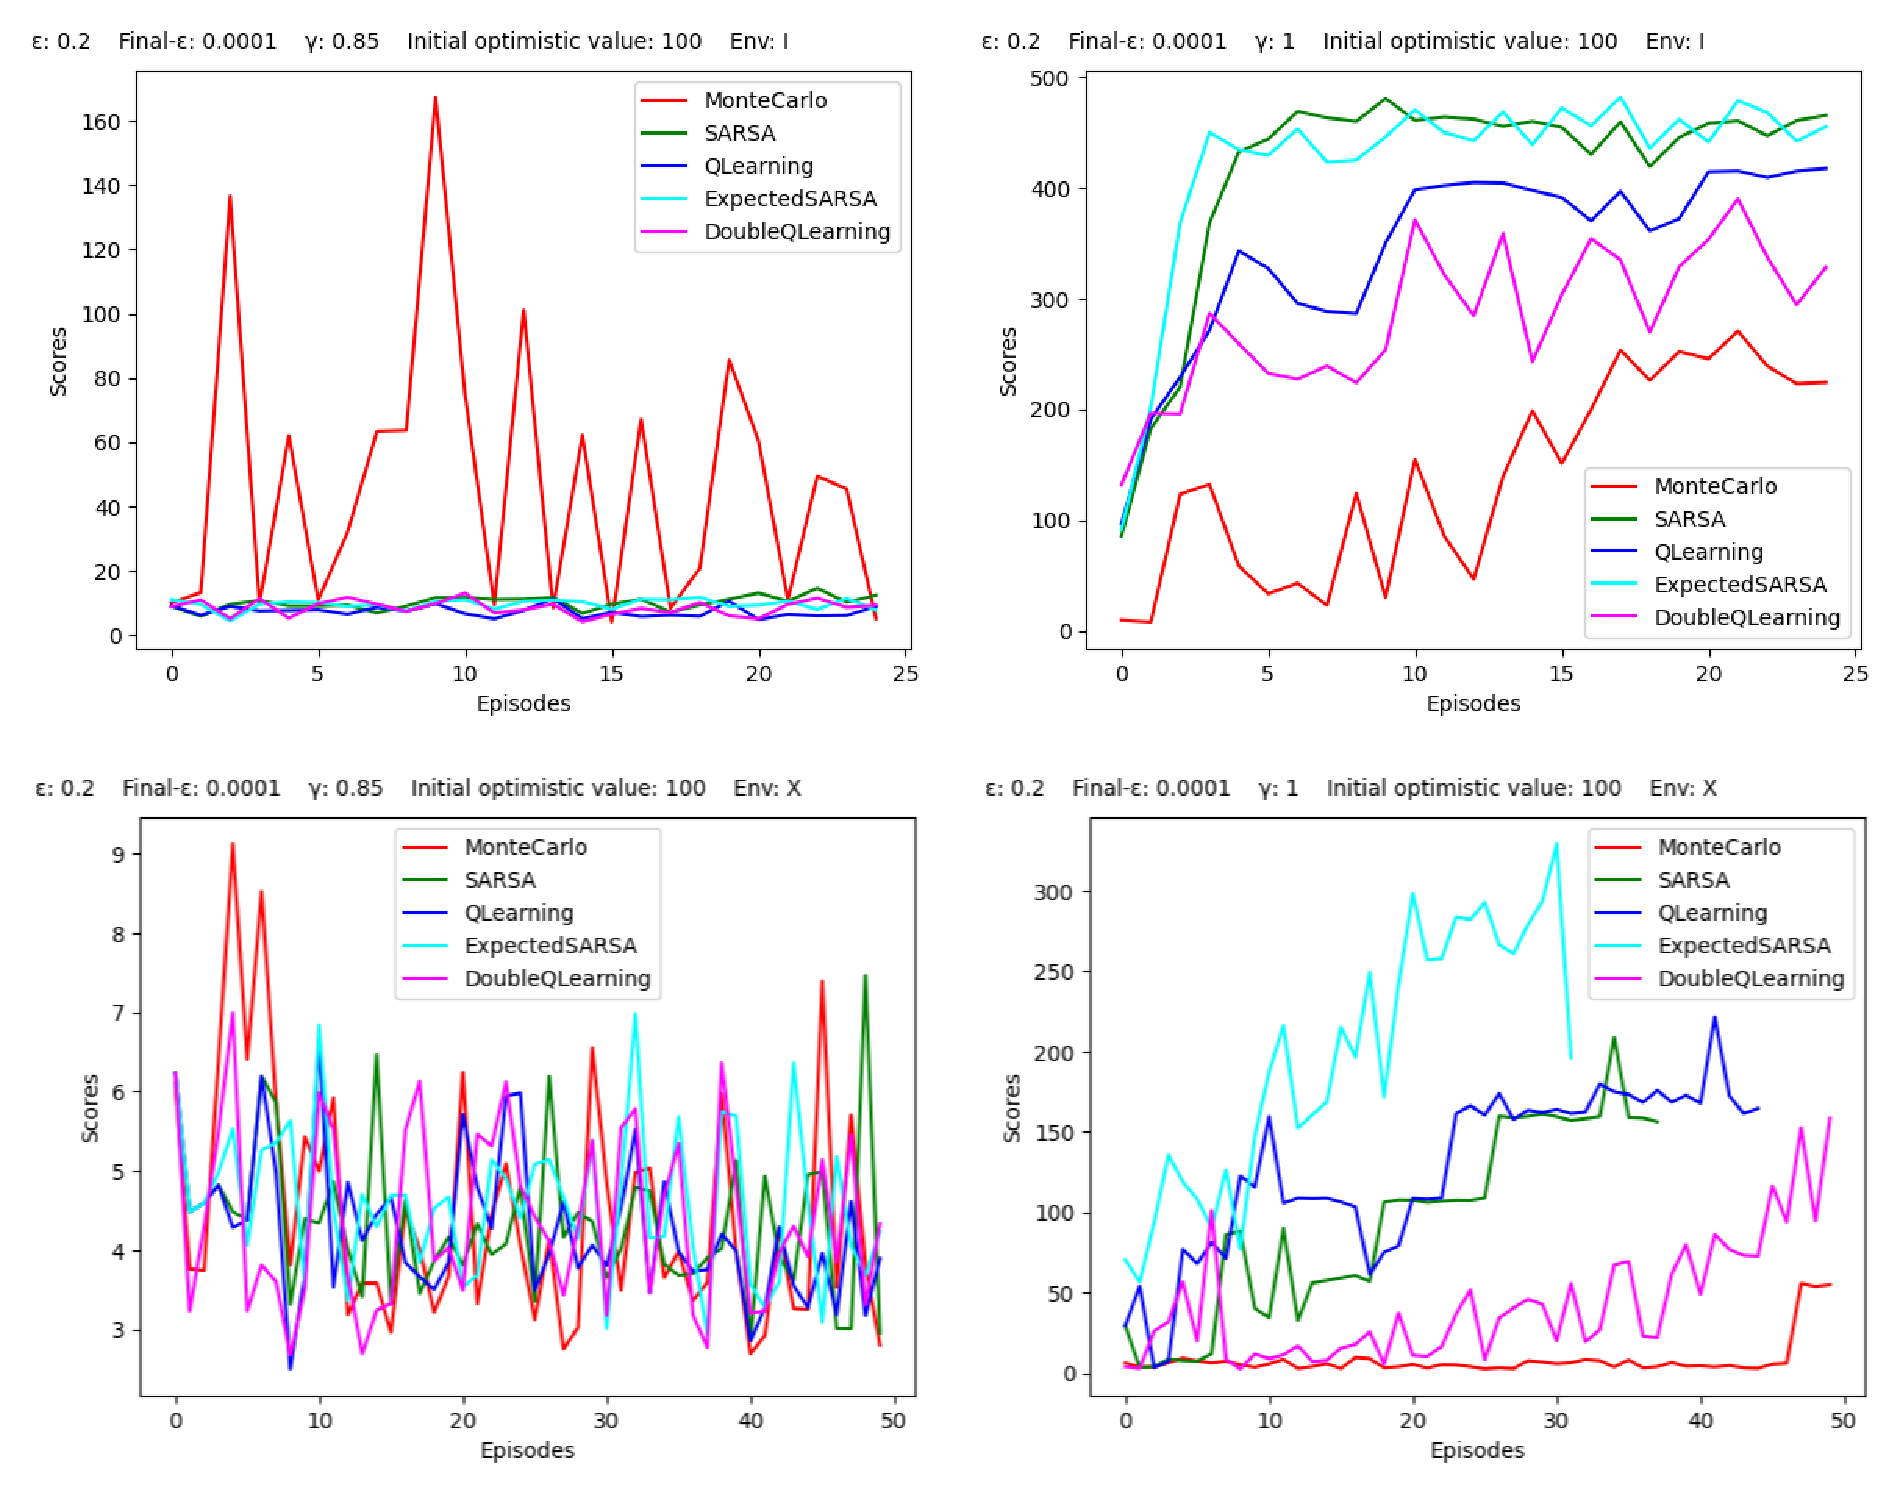
\includegraphics[width=\textwidth]{discountingExample}
    \caption{Full game with \texttt{ExpectedSARSA} example}
    \label{fig:full_game_es_eg}
\end{figure}

\section{Interesting behaviours}
\label{intbeh}
\begin{figure}[h]
    \centering
    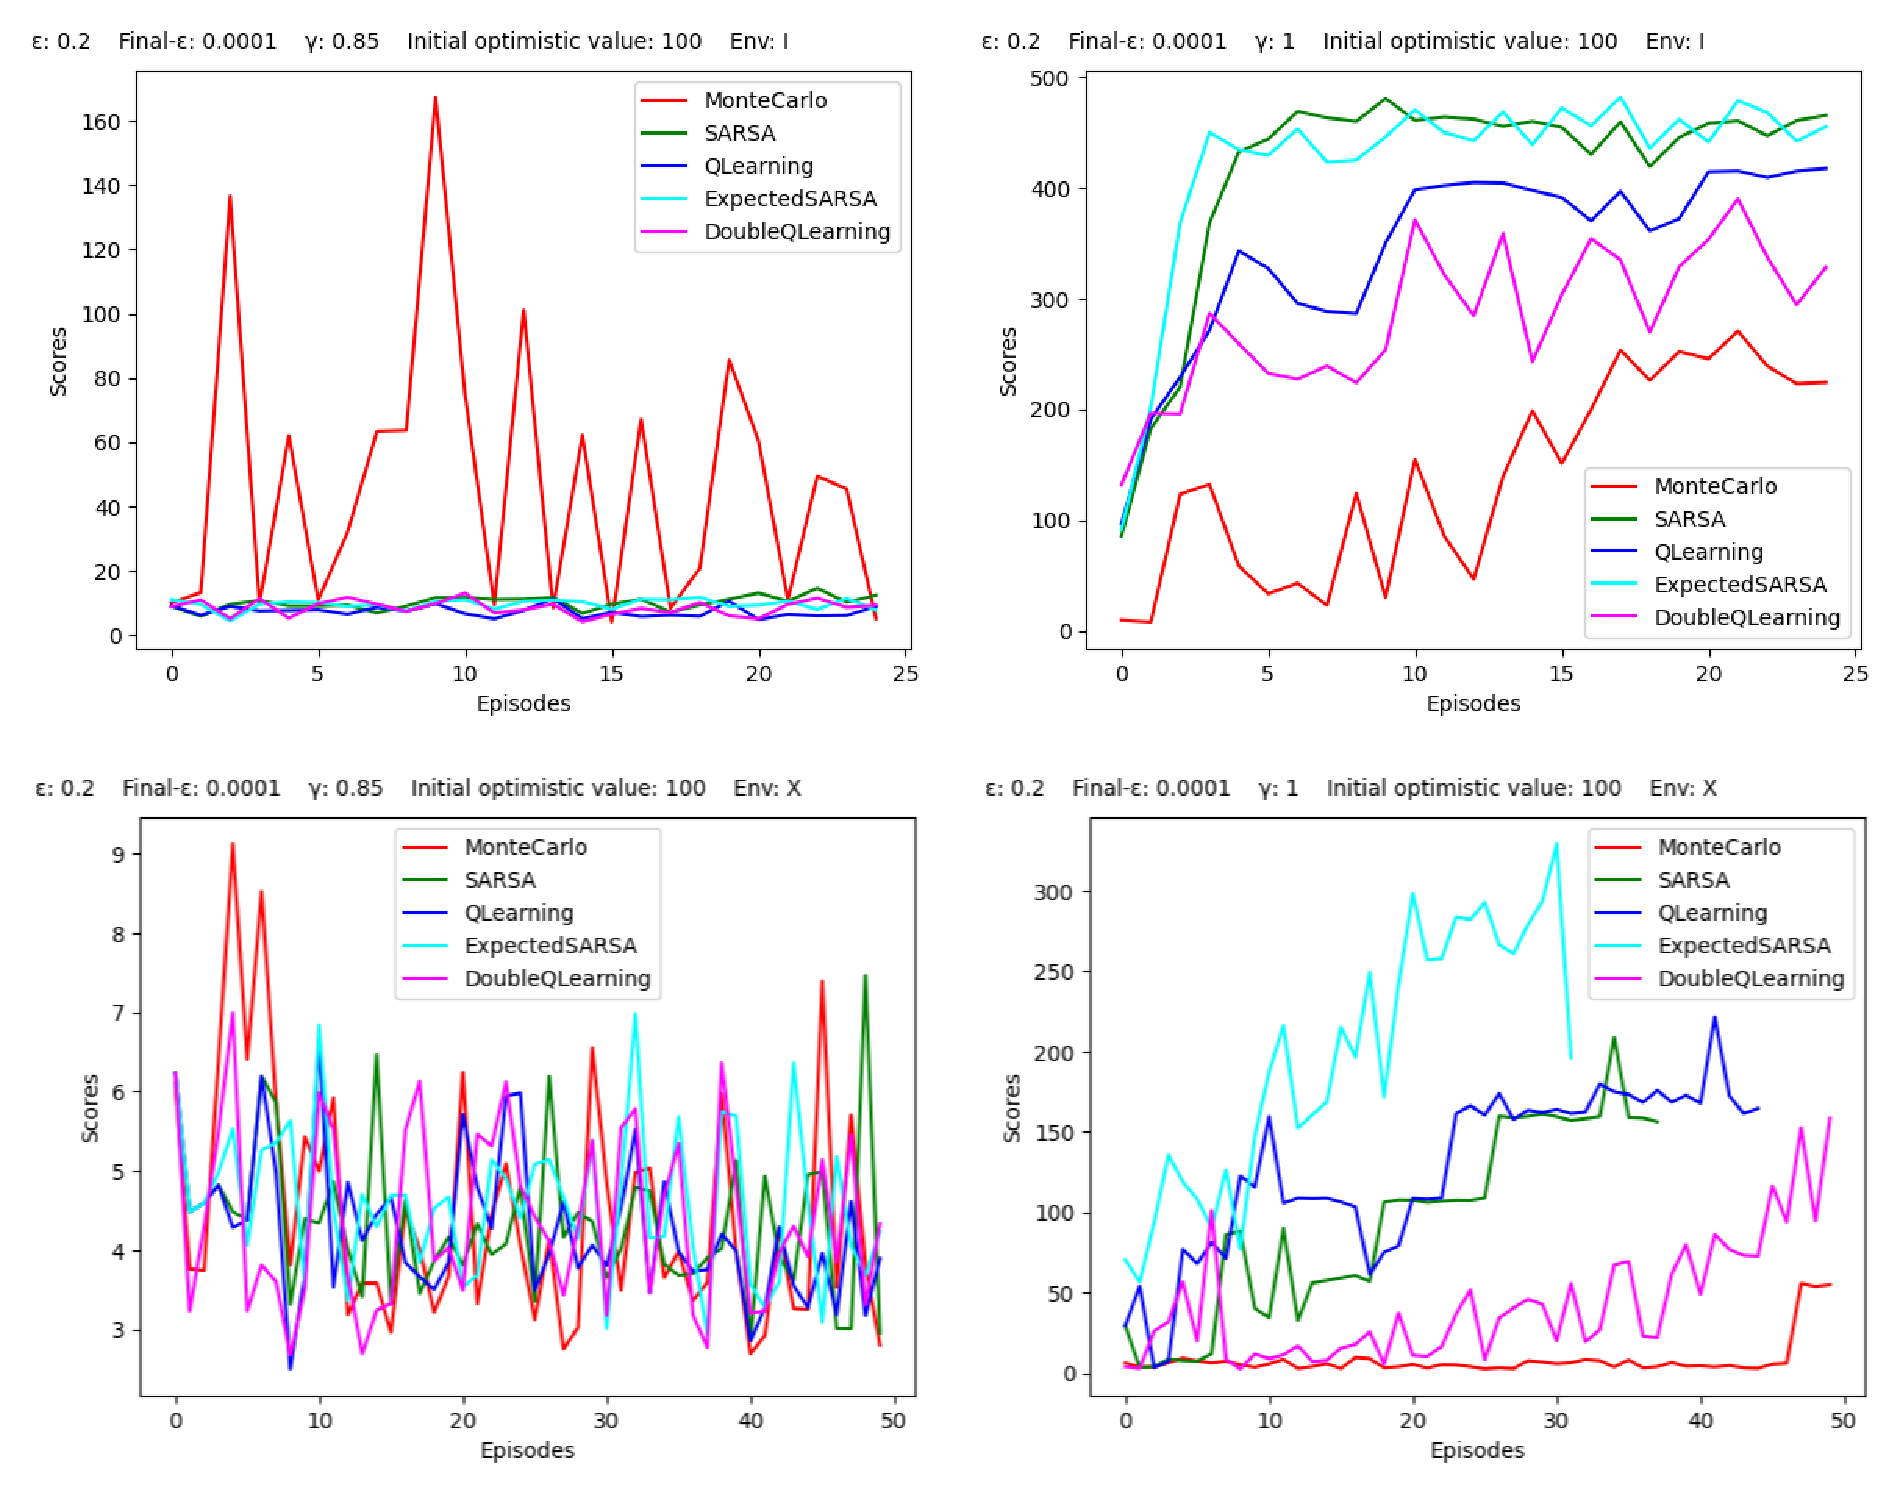
\includegraphics[width=\textwidth]{discountingExample}
    \caption{Discounting example}
    \label{fig:discounting_eg}
\end{figure}

In this chapter, we aim to discuss certain unexpected findings that surfaced during our experimentation. One of the immediate observations can be seen in Figure \ref{fig:discounting_eg}\footnote{No smoothing was applied to any of the plots in this subsection.}. We conducted experiments on two distinct environments, \texttt{env=[I]} and \texttt{env=[X]}, and for each environment, we carried out experiments with discount rates of \texttt{gam=0.85} and \texttt{gam=1.0} for all agents. As evident from the plots, the lower gamma value exhibited considerably poorer performance than when no discounting (\texttt{gam=1.0}) was applied. This trend is not limited to these specific environments and testing conditions but rather observed consistently across all our experimentation. This result is counter-intuitive since it seems logical that penalizing the last action more than previous ones would result in a better policy.

\begin{figure}[h]
    \centering
    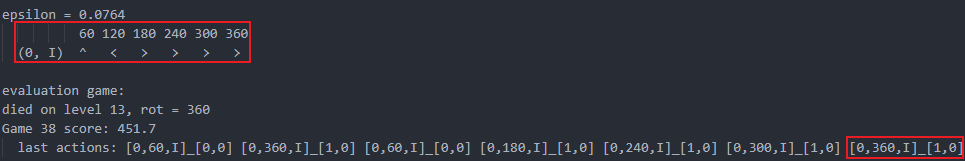
\includegraphics[width=\textwidth]{discountingExplanation}
    \caption{Discounting explanation}
    \label{fig:discounting_expl}
\end{figure}

Upon further investigation, we discovered that in some cases, a lost game for the agent does not result from the last action directly but rather from a chain reaction initiated by a previous bad decision. As seen in Figure \ref{fig:discounting_expl}, the agent's last action of going right at rotation \texttt{360} to reach a safe one, \texttt{60}, is not a poor decision in itself but rather the best possible action in that state\footnote{As confirmed by a human player, rotation 60 is safe for trap type I.}. However, analysing the last four actions taken by the agent, it becomes clear that it attempted to reach rotation \texttt{60} by going left from the rotation \texttt{180}. With a high score of \texttt{451.7} (Figure \ref{fig:discounting_eg}), the agent undeniably had high speed value, making it move forward very quickly, and while this policy may have been effective in the early game before the agent attained its current speed\footnote{It should recalled that after every 3 levels the agents speed increases.}, there is simply not enough time for the agent to rotate at this point in the game. In this case, one could argue that the fourth action from the last was responsible for the agent's loss. For cases like this, we believe that the agent performs better when all actions are penalized equally.

\begin{figure}[h]
    \centering
    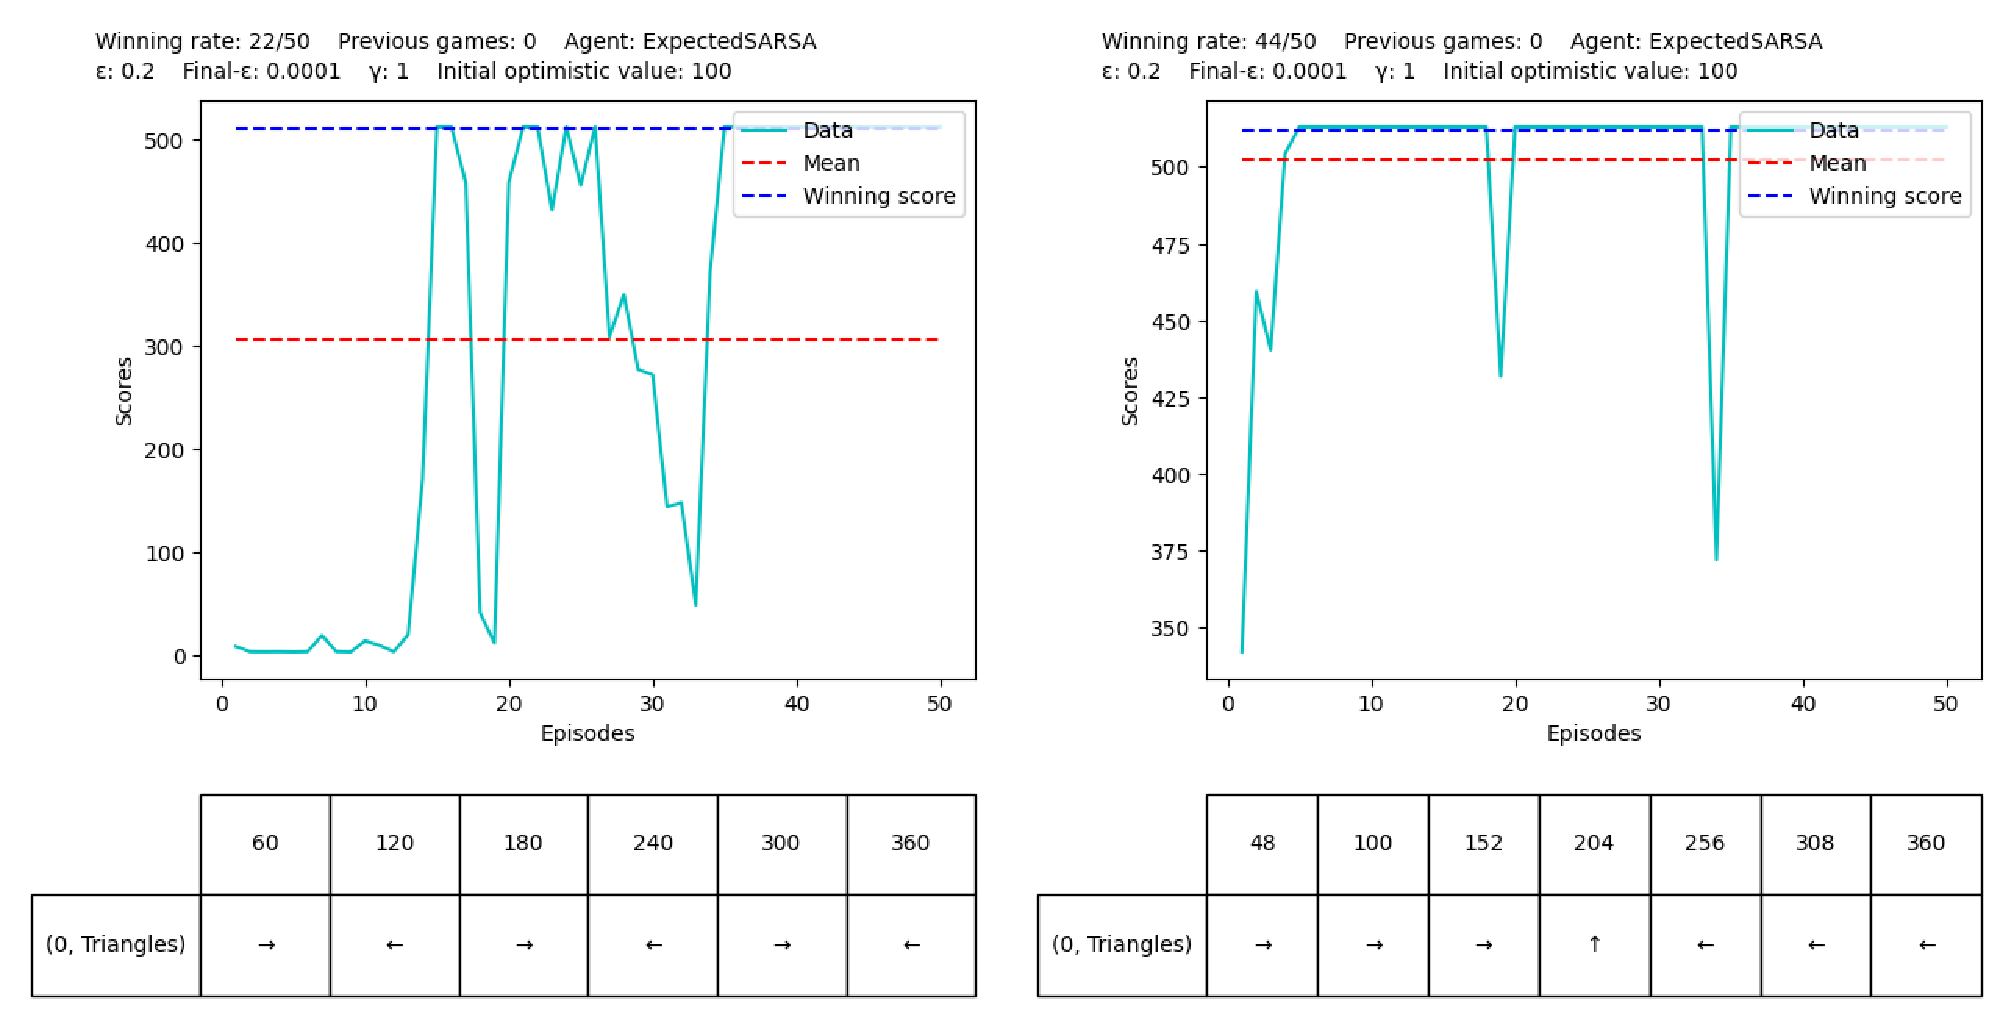
\includegraphics[width=\textwidth]{trianglesExample}
    \caption{\texttt{Triangles} example}
    \label{fig:triangles_intbeh_eg}
\end{figure}

Another intriguing behaviour emerged as a result of our learning architecture. As previously noted, we chose to have the agent not take a new action every time its \texttt{move()} function is called, but rather return the same action until the state changes. This resulted in a substantial reduction in the number of different actions taken by the agent, given that the move function is invoked every game tick, while state changes occur less frequently. This approach led to a behaviour that could not have been predicted at the outset. Figure \ref{fig:triangles_intbeh_eg} provides an illustration of this behaviour (with some sentiment \texttt{env=[Triangles]} was chosen as this was the first environment on which the behaviour was noticed).

Ordinarily, \texttt{env=[Triangles]} does not offer any safe rotations unless \texttt{rots=7} or more. As shown in the plot, the agent will certainly learn with this rotation value. However, if the agent is given only \texttt{6} rotation values to choose from, it will develop a policy that rapidly oscillates between two rotations, keeping the player character, Hans, on the edge of those rotations, allowing him to safely pass through the trap. This behaviour is not confined to situations where the agent is ``forced'' to make such a decision. During training, in many instances, the agent will learn to stay on the edge rather than advance into a completely safe rotation. There does not appear to be a preference for one or the other; rather, the policy the agent discovers first is determined by other experimental factors. It can be concluded that this behaviour arose solely because the agent did not alter its action until the state changed. In my opinion, this discovery is one of the most exciting outcomes of this project.